\begin{anexosenv}

\partanexos

\chapter{Termo de Abertura do Projeto}

  % \documentclass[12pt,openright,oneside,a4paper,brazil]{abntex2}
% \usepackage[utf8]{inputenc}
% \counterwithout{section}{section}
% \counterwithout{figure}{chapter}
% \counterwithout{table}{chapter}
% \setlength{\parindent}{1.3cm}
% \usepackage{indentfirst}
% \setlength{\parskip}{0.2cm}
% \usepackage[bottom=2cm,top=3cm,left=3cm,right=2cm]{geometry}
% \usepackage{graphicx}
% \graphicspath{{figuras/}}
% \usepackage{placeins}
% 
% %opening
% \title{}
% \author{}
% 
% \begin{document}

%capa

% \textual
\begin{center}
 {\large Termo de abertura}\\[0.2cm]
 {Planta de abastecimento de água potável a partir da umidade do ar}\\
 \end{center}
 
 \section*{Histórico de Alterações}
\begin{table}[h]
\centering
\begin{tabular}{|c|c|p{6cm}|p{5cm}|}

Data & Versão & Descrição & Responsável\\
\hline                               
20/04/2015 & 0.0 & Criação do documento pelo grupo de integração. & Ludimila S. Ferreira,
Laís R. Carvalho, Rafael C. Bragança, Vitor Silva.\\
\hline
21/04/2015 & 1.0 & Alteração dos itens: III, IV,V,VI,VII,VIII(3), IX & Ludimila S. Ferreira,
Laís R. Carvalho, Rafael C. Bragança, Vitor Silva.\\
\hline
\end{tabular}
\end{table}

\section*{Nome do projeto}
  Planta de abastecimento de água potável a partir da umidade do ar
  
  \section*{Descrição do projeto}
O projeto visa desenvolver uma planta de abastecimento de água potável, por meio de um sistema de captação a partir da umidade do ar na cidade de Aracari-RN (município da Microrregião do Seridó Oriental, na região do Seridó), no bairro Vereador Tarcísio Bezerra Galvão. O bairro possui uma população de aproximadamente 900 habitantes e sofre constantemente com a falta de água. 
O projeto gira em torno de uma solução tecnológica  capaz de retirar a água do ar e por processos químicos e físicos e tornar essa água potável e própria para o consumo humano de forma renovável e menos danosa possível. Para isso aplicamos conhecimentos das demais áreas da engenharia atuando no desenvolvimento e conceituação do projeto. Nossa estimativa é de que possamos produzir aproximadamente 3 mil litros de água por dia. Essa quantidade e suficiente para atender toda a população do município. 
O projeto conta com grupos que trabalham em áreas diferentes mas interligadas e com um único propósito. Cada etapa e gerida e coordenada por representantes de forma a garantir um resultado rápido e com qualidade.


\section*{Objetivos do projeto}
  
  Este trabalho tem por objetivo propor um projeto de solução que consiga suprir a demanda da população. Os esforços que serão
realizados ao longo do período de desenvolvimento, no transcorrer de todas as etapas do processo buscam a qualidade e real
eficácia do produto, ou seja, oferecer a demanda de água do bairro Vereador Tarcísio Bezerra Galvão situado em Aracarí-RN, 
água potável de qualidade.

 São objetivos específicos do projeto:
 \begin{itemize}
  \item Elaborar o projeto mecânico estrutural do sistema de captação de água;
  \item Elaborar o projeto estrutural do sistema de transporte da água para a central de armazenamento;
  \item Elaborar o projeto do sistema de monitoramento e controle da qualidade da água captada;
  \item Elaborar o projeto da matriz energética que dará o suporte para os sistemas de captação de água e monitoramento e controle;
 \end{itemize}
  
\section*{Justificativa do projeto}
 \begin{enumerate}[label=\Alph*]
\item Por que deve-se pensar em projetos como esse?\\
Atualmente, cerca de 40 \% da população mundial sofre com consequências da falta de água, além da sede faltam recursos hídricos, o que gera graves implicações na economia e política. De acordo com o geólogo Sjiklomanov, do Instituto Hidrológico Estadual de São Petesburgo, Rússia, em 2000 foi previsto que: “Os países em desenvolvimento vão aumentar seu uso de água em até 200\% em 25 anos”. Em 2014 no Brasil, foi evidenciado consequências desse aumento no consumo de água juntamente com fatores climático, resultando na falta de água em cidades de Pernambuco, Minas Gerais e São Paulo.
Essa situação de falta de água não é nova, a ONU em 2003 já previa os futuros transtornos que seriam causados pela crise de água. O World Water Development Report, se destaca sobre o tema porque é um documento da ONU que também traz estudos mostrando como esse problema já afeta e mata milhares de pessoas. Este estudo prevê que 2,7 bilhões de seres humanos – 45\% da população mundial – vão ficar sem água no ano 2025.
Diante dessa situação e de previsões sobre a falta de água tão breves, devem-se tomar medidas para minimizar a situação e planejar soluções para a produção de água potável buscando outras fontes, como o ar, por exemplo. Por isso, esse projeto visa através da umidade do ar, retirar água potável e planeja um estudo de abastecimento na cidade de Acari, RN.

\item Por que  Aracarí foi a cidade escolhida?\\
Na situação de crise hídrica vivida pelo país atualmente, observa-se grandes centros urbanos sofrendo com a falta de água para consumo humano (o que antes era praticamente exclusivo para a região do semiárido nordestino). Além disso, observa-se que a seca na região nordeste vem se agravando muito nos últimos anos, especificamente na região do Seridó, que fica no semiárido do RN.
Dessa forma, soluções alternativas para o abastecimento de água potável a fim de atender o consumo humano fazem-se necessárias. Sendo assim, a região para a qual o sistema será projetado será o município de Acari – RN, pois é uma região onde há muita demanda (11303 habitantes) e tem sofrido muito com a escassez de água. A escolha dessa região baseia-se principalmente na questão social, uma vez que o projeto visa atender o consumo humano de pessoas que não tem acesso à água potável.
Além de ser uma região que apresenta necessidade de um planejamento para a amenização ou suprimento da escassez de água, é também, uma região muito quente com temperatura média anual de 33Cº, pois está localizada no polígono das Secas (local de maior concentração de seca no país). Consequentemente, o volume de água do Açude de Gargalheiras, açude este que abastece a cidade, decai consideravelmente em épocas de seca, fazendo com que haja escassez de água na cidade. A possibilidade de retirar água potável do subterrâneo, é inviável pois a água é muito salobra. Apesar de clima quente e semi-árido a umidade do ar nessa região  possui uma média anual de 60\%, o que possibilita a implantação de tecnologias que retiram a umidade do ar  e transforma em água potável. Portanto, devido a esses fatores apresentados, a cidade foi escolhida para se realizar o planejamento.

\item Por que se escolheu o bairro Vereador Tarcísio Bezerra Galvão?\\
De acordo com o censo 2010 o bairro Vereador Tarcísio Bezerra Galvão tem cerca de 900 habitantes onde a maioria, cerca de 60\%, possui entre 15 e 64 anos. Sua localização foi uma das principais motivações para a escolha do bairro, pois é um bairro muito próximo do Açude de Gargalheiras, e uma das áreas a ser planejada nesse projeto é em relação à distribuição da água, ou seja, o açude pode facilitar essa distribuição. Outro motivo seria para limitar um pouco mais o projeto a uma população menor, para assim agilizar e facilitar o estudo para planejamento.
\end{enumerate}
  
\section*{Nome do gerente do projeto, suas responsabilidades e sua autoridade }
Gerente de Projeto – Adrianny Viana de Araújo Amorim: responsável pelo projeto; realizar a gestão da mudança, escopo, custo, qualidade e os recursos que serão compartilhados entre os vários setores do projeto; selecionar e adaptar os processos de gerenciamento de projetos mais apropriados para a realidade da gerência, na medida da necessidade; dirigir e liderar a equipe, almejando a realização dos objetivos e metas; acompanhar a maturidade da equipe em gerenciamento de projetos, identificando necessidades de orientação e treinamentos; aprovar o plano de cada parte do projeto e autoriza sua execução; definir documentos padrões, base de dados e ferramentas; convocar e coordenar reuniões do projeto; administrar conflitos; definir o escopo do produto.

\section*{Necessidades básicas do trabalho a ser realizado }
Para a realização do projeto é necessária uma boa gestão para que todos os envolvidos tenham o máximo de aproveitamento do tempo dedicado. Organização e cumprimento de prazos bem como respeito as lideranças escolhidas. E extremamente importante que o trabalho seja realizado em um ambiente favorável ao desenvolvimento de ideias e que possua recursos que visem possibilitar e facilitar o andamento do projeto. O acesso a internet e indispensável para que possamos manter uma comunicação rápida e eficaz. A utilização de computadores ajuda no tempo de execução das tarefas, possibilitando pesquisas mais rápidas e um melhor gerenciamento das informações do projeto.
Aliado a tudo descrito a cima, a competência de toda a equipe em suas áreas de atuação.


\section*{Detalhes do projeto}
\begin{enumerate}
\item Produto do projeto
\begin{itemize}
\item Projeto estrutural mecânico das unidades de captação de água da umidade do ar.
\item Projeto estrutural do sistema de transporte da água para a central de armazenamento.
\item Projeto do sistema de monitoramento e controle da qualidade da água captada.
\item Projeto da matriz energética que dará o suporte para os sistemas de captação de água e monitoramento e controle.
\end{itemize}
\item Cronograma de marcos sumarizado 
\begin{itemize}
\item Pesquisa sobre tecnologias de captação da água inicio 25/03/2015
\item Pesquisar sobre local para a implantação do projeto 25/03/2015 
\item Pesquisar informações sobre o local (clima, tempo, população...)30/03/201
\item Pesquisar sobre localidade específica  06/04/2015
\item Fazer análise do escopo (5W/2H) 13/04/2015
\item Criar Termo de abertura do projeto 20/04/2015
\item Fazer Declaração de escopo 17/04/2015
\item Fazer Relatório do projeto 17/04/2015
\item Ponto de controle 2   30/04/2015
\item Ponto de controle 3   26/05/2015
\end{itemize}
\item Estimativas iniciais de custos \ \\
	Será necessário um investimento na casa dos milhares. Foi levado em conta suporte legal e tributário, suprimentos de escritório, equipamentos, despesas postais, espaço administrativo, salário dos funcionários, entre outros fatores. Com isso temos uma necessidade inicial de aproximadamente R\$ 800 mil, previsto um tempo de implementação de 6 meses.
\end{enumerate}

\section*{Administração}
\begin{enumerate}
\item Necessidade inicial de recursos\\
O projeto conta com uma distribuição recursos humanos composta da seguinte forma: 
\begin{itemize}
\item Escopo
\item Qualidade
\item Tempo
\item Integração
\item Custo
\item Comunicação
\item Risco
\item RH
\item Aquisição
\end{itemize}
Cada área possui aproximadamente 3 membros, somando um total de 25 membros na equipe. Dentre as áreas citadas temos a distribuição do pessoal de acordo afinidade e competência estabelecidos. Os membros de cada um dos grupos vem das áreas de Engenharias de Software; Energia; Automotiva; Eletrônica; e Aeroespacial. Também serão necessários profissionais das áreas de engenharia mecânica, engenharia de redes ,advocacia e química dada a necessidade no projeto de conhecimentos específicos nessas áreas.\\
Para equipamentos: computadores, acesso a internet, softwares de gerenciamento, pacote office, acesso a impressão, armazenamento e transporte de dados, local físico para reuniões, suprimentos de escritório ( caneta, papel, quadro branco, pincel para quadro branco, mesa, cadeiras, calculadoras).
\item Necessidade de suporte pela organização\\
Temos a necessidade do apoio de especialistas, na forma de consultoria, nas áreas do conhecimento requisitadas pelo projeto. Os especialistas nos ajudarão com dando uma visão mais critica e coesa sobre determinados aspectos a serem implementados ou direções a serem tomadas no andamento do projeto.

\end{enumerate}
\newpage
\section*{Assinaturas}
\begin{center}
Data: \rule{0.5cm}{0.1mm}/\rule{0.5cm}{0.1mm}/\rule{1cm}{0.1mm}     \\
\rule{13cm}{0.1mm}\\
ADRIANNY VIANA DE ARAÚJO AMORIM – GERENTE DE PROJETO\\


\end{center}
% \end{document}
  
\chapter{Declaração de Escopo}

  % \documentclass[12pt,openright,oneside,a4paper,brazil]{abntex2}
% \usepackage[utf8]{inputenc}
% \counterwithout{section}{section}
% \counterwithout{figure}{chapter}
% \counterwithout{table}{chapter}
% \setlength{\parindent}{1.3cm}
% \usepackage{indentfirst}
% \setlength{\parskip}{0.2cm}
% \usepackage[bottom=2cm,top=3cm,left=3cm,right=2cm]{geometry}
% \usepackage{graphicx}
% \graphicspath{{figuras/}}
% \usepackage{placeins}
% 
% %opening
% \title{}
% \author{}
% 
% \begin{document}

%capa

% \textual
\begin{center}
 {\large Declaração de escopo}\\[0.2cm]
 {Planta de abastecimento de água potável a partir da umidade do ar}\\
 \end{center}
 
 \section*{Histórico de Alterações}
\begin{table}[h]
\centering
\begin{tabular}{|c|c|p{6cm}|p{5cm}|}

\hline
Data & Versão & Descrição & Responsável\\
\hline                               
21/04/2015 & 0.0 & Criação do documento. & César A. Marques Jr., Jonnatas L.L. Costa\\
\hline
22/04/2015 & 1.0 & Alteração dos itens: III, VII e IX & Jonnatas L. L. Costa\\
\hline
22/04/2015 & 1.1 & Alteração dos requisitos & Jonnatas L. L. Costa\\
\hline
\end{tabular}
\end{table}

\section*{Nome do projeto}
  Planta de abastecimento de água potável a partir da umidade do ar
  
  \section*{Descrição do projeto}
O projeto visa desenvolver uma planta de abastecimento de água potável, por meio de um sistema de captação a partir da umidade do ar na cidade de Aracari-RN (município da Microrregião do Seridó Oriental, na região do Seridó), no bairro Vereador Tarcísio Bezerra Galvão. O bairro possui uma população de aproximadamente 900 habitantes e sofre constantemente com a falta de água. 
O projeto gira em torno de uma solução tecnológica  capaz de retirar a água do ar e por processos químicos e físicos e tornar essa água potável e própria para o consumo humano de forma renovável e menos danosa possível. Para isso aplicamos conhecimentos das demais áreas da engenharia atuando no desenvolvimento e conceituação do projeto. Nossa estimativa é de que possamos produzir aproximadamente 3 mil litros de água por dia. Essa quantidade e suficiente para atender toda a população do município. 
O projeto conta com grupos que trabalham em áreas diferentes mas interligadas e com um único propósito. Cada etapa e gerida e coordenada por representantes de forma a garantir um resultado rápido e com qualidade.


\section*{Objetivos do projeto}
  
  Este trabalho tem por objetivo propor um projeto de solução que consiga suprir a demanda da população. Os esforços que serão
realizados ao longo do período de desenvolvimento, no transcorrer de todas as etapas do processo buscam a qualidade e real
eficácia do produto, ou seja, oferecer a demanda de água do bairro Vereador Tarcísio Bezerra Galvão situado em Aracarí-RN, 
água potável de qualidade.

 São objetivos específicos do projeto:
 \begin{itemize}
  \item Elaborar o projeto mecânico estrutural do sistema de captação de água;
  \item Elaborar o projeto estrutural do sistema de transporte da água para a central de armazenamento;
  \item Elaborar o projeto do sistema de monitoramento e controle da qualidade da água captada;
  \item Elaborar o projeto da matriz energética que dará o suporte para os sistemas de captação de água e monitoramento e controle;
 \end{itemize}
  
\section*{Justificativa do projeto}
 \begin{enumerate}[label=\Alph*]
\item Por que deve-se pensar em projetos como esse?\\
Atualmente, cerca de 40 \% da população mundial sofre com consequências da falta de água, além da sede faltam recursos hídricos, o que gera graves implicações na economia e política. De acordo com o geólogo Sjiklomanov, do Instituto Hidrológico Estadual de São Petesburgo, Rússia, em 2000 foi previsto que: “Os países em desenvolvimento vão aumentar seu uso de água em até 200\% em 25 anos”. Em 2014 no Brasil, foi evidenciado consequências desse aumento no consumo de água juntamente com fatores climático, resultando na falta de água em cidades de Pernambuco, Minas Gerais e São Paulo.
Essa situação de falta de água não é nova, a ONU em 2003 já previa os futuros transtornos que seriam causados pela crise de água. O World Water Development Report, se destaca sobre o tema porque é um documento da ONU que também traz estudos mostrando como esse problema já afeta e mata milhares de pessoas. Este estudo prevê que 2,7 bilhões de seres humanos – 45\% da população mundial – vão ficar sem água no ano 2025.
Diante dessa situação e de previsões sobre a falta de água tão breves, devem-se tomar medidas para minimizar a situação e planejar soluções para a produção de água potável buscando outras fontes, como o ar, por exemplo. Por isso, esse projeto visa através da umidade do ar, retirar água potável e planeja um estudo de abastecimento na cidade de Acari, RN.

\item Por que  Aracarí foi a cidade escolhida?\\
Na situação de crise hídrica vivida pelo país atualmente, observa-se grandes centros urbanos sofrendo com a falta de água para consumo humano (o que antes era praticamente exclusivo para a região do semiárido nordestino). Além disso, observa-se que a seca na região nordeste vem se agravando muito nos últimos anos, especificamente na região do Seridó, que fica no semiárido do RN.
Dessa forma, soluções alternativas para o abastecimento de água potável a fim de atender o consumo humano fazem-se necessárias. Sendo assim, a região para a qual o sistema será projetado será o município de Acari – RN, pois é uma região onde há muita demanda (11303 habitantes) e tem sofrido muito com a escassez de água. A escolha dessa região baseia-se principalmente na questão social, uma vez que o projeto visa atender o consumo humano de pessoas que não tem acesso à água potável.
Além de ser uma região que apresenta necessidade de um planejamento para a amenização ou suprimento da escassez de água, é também, uma região muito quente com temperatura média anual de 33Cº, pois está localizada no polígono das Secas (local de maior concentração de seca no país). Consequentemente, o volume de água do Açude de Gargalheiras, açude este que abastece a cidade, decai consideravelmente em épocas de seca, fazendo com que haja escassez de água na cidade. A possibilidade de retirar água potável do subterrâneo, é inviável pois a água é muito salobra. Apesar de clima quente e semi-árido a umidade do ar nessa região  possui uma média anual de 60\%, o que possibilita a implantação de tecnologias que retiram a umidade do ar  e transforma em água potável. Portanto, devido a esses fatores apresentados, a cidade foi escolhida para se realizar o planejamento.

\item Por que se escolheu o bairro Vereador Tarcísio Bezerra Galvão?\\
De acordo com o censo 2010 o bairro Vereador Tarcísio Bezerra Galvão tem cerca de 900 habitantes onde a maioria, cerca de 60\%, possui entre 15 e 64 anos. Sua localização foi uma das principais motivações para a escolha do bairro, pois é um bairro muito próximo do Açude de Gargalheiras, e uma das áreas a ser planejada nesse projeto é em relação à distribuição da água, ou seja, o açude pode facilitar essa distribuição. Outro motivo seria para limitar um pouco mais o projeto a uma população menor, para assim agilizar e facilitar o estudo para planejamento.
\end{enumerate}
  
\section*{Produtos do projeto}

  O presente trabalho fornecerá os seguintes produtos:
  
  \begin{itemize}
    \item Projeto estrutural mecânico das unidades de captação de água da umidade do ar.
    \item Projeto estrutural do sistema de transporte da água para a central de armazenamento.
    \item Projeto do sistema de monitoramento e controle da qualidade da água captada.
    \item Projeto da matriz energética que dará o suporte para os sistemas de captação de água e monitoramento e controle.
  \end{itemize}

\section*{Critérios de aceitação do produto do projeto}

  Os produtos de projeto devem atender as especificações inerentes aos requisitos funcionais
  e não-funcionais de cada produto específico.
  
\section*{Exclusões específicas e limites do projeto}

  Ficam excluídos das competências do projeto:
  
  \begin{itemize}
   \item Atividades como as de tratamento de recursos hídricos já existentes na região e que não possuem
      as especificações mínimas para consumo humano, como é o caso da água salobra.
   
   \item Todo o processo de manutenção dos componentes do sistema, visando uma durabilidade de longo prazo, não fará parte 
      do escopo deste projeto. Também não fará parte do escopo a distribuição de água para localidades vizinhas.
      
   \item O uso de tecnologias auxiliares para a obtenção da água, como é o caso osmose reversa, não serão abordadas
      pois fogem da premissa inicial.
   
   \item O tratamento da energia residual gerada.
   
   \item O tratamento da água residual que for armazenada nos tanques.
   
  \end{itemize}

\pagebreak
\section*{Estrutura Analítica do Projeto}

  \begin{figure}[h]
  \begin{center}
    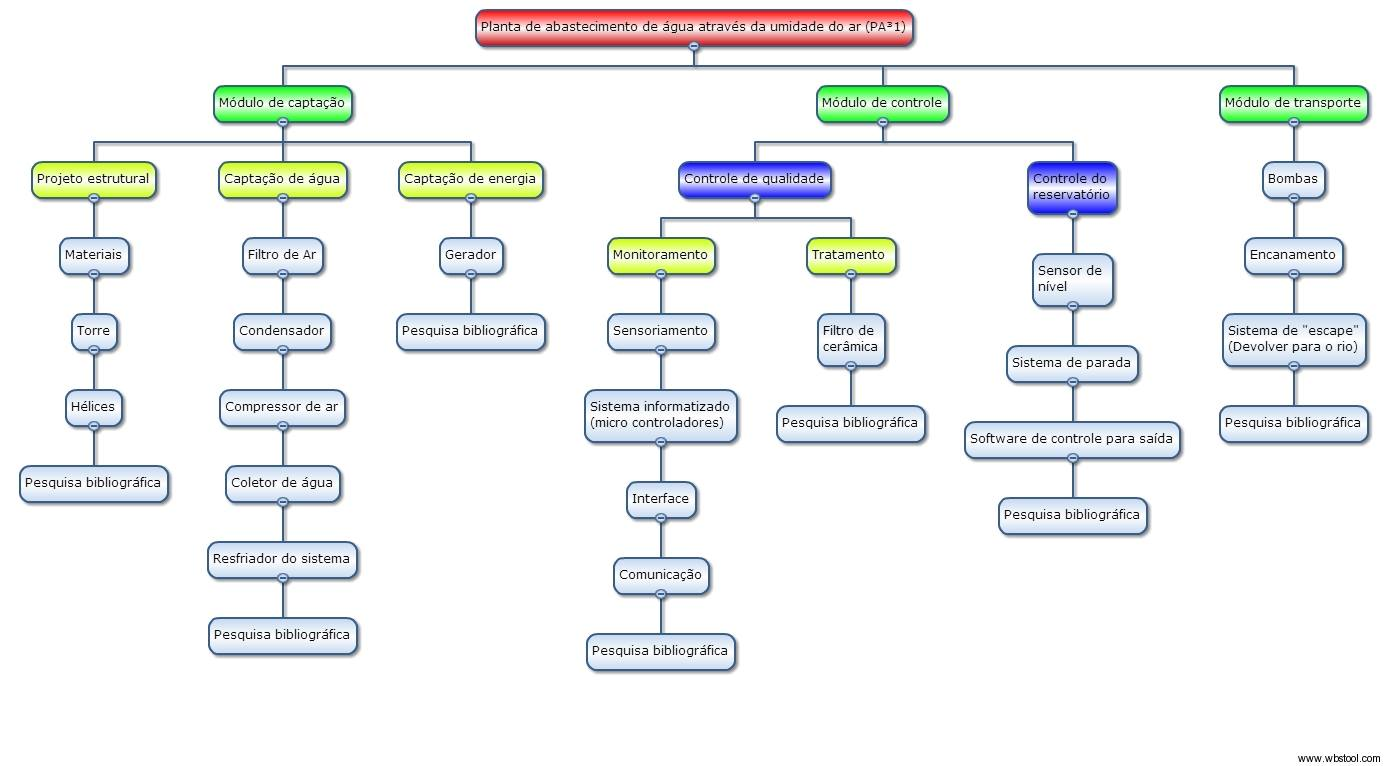
\includegraphics[scale=0.3]{editaveis/figuras/EAP}
    \label{EAP}
  \end{center}
  \end{figure}
  \FloatBarrier
  
\section*{Características e requisitos do produto do projeto}

  Os produtos do projeto são partes que compõem um sistema que tem por características principais ser um sistema auto sustentável
  e que não seja muito agressivo ao meio ambiente, utilizando uma matriz energética alternativa.
  A estimativa é que o produto gere cerca de 3 mil litros de água potável por dia.
  
  O sistema conta com uma central de monitoramento para garantir a qualidade da água produzida. Possui uma série de sensores
  com funções variadas, que vão de ler a umidade do ar até a medição de dados sobre a água.
  
  Uma importante característica do sistema é que ele pode se adequar às mudanças climáticas, de forma que ele pare de
  funcionar quando a umidade do ar chegar a um nível mínimo, para que não afete a saúde da população.
  
  O projeto possui quatro frentes de requisitos:
  
    \begin{itemize}
      \item Requisitos do projeto estrutural mecânico do sistema de captação da água e do transporte para a central de armazenamento;\\
	
	\textbf{Requisitos funcionais}
	\begin{itemize}
	  \item 
	\end{itemize}
	
	\textbf{Requisitos não-funcionais}
	\begin{itemize}
	  \item 
	\end{itemize}
	
      \item Requisitos do projeto dos circuitos eletrônicos que irão compor o sistema de monitoramento e controle da qualidade da água.\\
	
	\textbf{Requisitos funcionais}
	\begin{itemize}
	  \item Atuar como um sistema de controle dos elementos do sistema de modo a produzir a saída desejada (manter a água própria para o consumo humano);
	  \item Obter informações climáticas da região;
	  \item Obter dados do estado reservatório;
	  \item Ler parâmetros que definem a qualidade da água;
	  \item Efetuar conversão analógica/digital dos sinais filtrados;
	  \item Processar o sinal convertido de modo que os dados possam ser transmitidos ao usuário;
	  \item Exibir dados obtidos ao usuário;
	\end{itemize}
	
	\textbf{Requisitos não-funcionais}
	\begin{itemize}
	  \item Utilizar sensores para obtenção dos dados;
	  \item Exibir dados dos sensores ao usuário em tempo real;
	  \item Utilizar filtros analógicos para retirar eventuais ruídos que a saída do sensor possa gerar;
	\end{itemize}
	
      \item Requisitos do projeto do sistema de Gestão da Informação do monitoramento da qualidade da água;\\
	 
	 \textbf{Requisitos funcionais}
	  \begin{itemize}
	   \item Apenas o moderador poderá, modificar os dados.
	   \item O sistema registrará os dados de qualidade da agua.
	   \item O sistema deve emitir um alerta caso um parâmetro de qualidade não esteja aceitável.
	   \item O sistema deve permitir consultas dos dados armazenados de datas anteriores.
	   \item O sistema deve possuir uma interface pare exibir os dados.
	   \item O sistema deve possuir uma página de \textit{login} antes de entrar no sistema.
	   \item O sistema deve possuir um mecanismo de impressão dos dados.
	   \item O sistema possuirá um mecanismo para exportar os dados.
	  \end{itemize}
	  
	  \textbf{Requisitos não-funcionais}
	  \begin{itemize}
	   \item O sistema deve ser fácil de usar, evitando excesso de digitação, de modo a dar agilidade ao processo.
	   \item O sistema deve possuir uma interface simples.
	   \item O sistema deve funcionar no sistema operacional Windows.
	   \item O sitema deve monitorar as amostras de água a cada 30 mimutos.
	  \end{itemize}
      
      \item Requisitos do projeto da matriz energética que dará o suporte para o sistema de captação de água e o sistema de monitoramento da qualidade da água;\\
      
	\textbf{Requisitos funcionais}
	\begin{itemize}
	  \item Produzir energia elétrica através da energia eólica;
	  \item Converter energia cinética em energia elétrica;
	  \item Armazenar a energia elétrica gerada;
	  \item Fornecer energia para os componentes eletrônicos, de controle e monitoramento do produto final;
	  \item Fornecer energia para o bombeamento mecânico de água.
	\end{itemize}
	
	\textbf{Requisitos não-funcionais}
	\begin{itemize}
	  \item Utilizar uma fonte renovável de energia;
	  \item Ser autossuficiente no quesito energia gerada-consumida;
	  \item Possuir eficiência energética aceitável;
	  \item Ser estável energeticamente;
	\end{itemize}
	
    \end{itemize}
  
\section*{Assinaturas}

  \begin{center}
  Data: \rule{0.5cm}{0.1mm}/\rule{0.5cm}{0.1mm}/\rule{1cm}{0.1mm}     \\
  \rule{13cm}{0.1mm}\\
  ADRIANNY VIANA DE ARAÚJO AMORIM – GERENTE DE PROJETO\\


\end{center}
% \end{document}

\chapter{Plano de Gerenciamento do Projeto}

  % \documentclass[12pt,openright,oneside,a4paper,brazil]{abntex2}
% \usepackage[utf8]{inputenc}
% \counterwithout{section}{section}
% \counterwithout{figure}{chapter}
% \counterwithout{table}{chapter}
% \setlength{\parindent}{1.3cm}
% \usepackage{indentfirst}
% \setlength{\parskip}{0.2cm}
% \usepackage[bottom=2cm,top=3cm,left=3cm,right=2cm]{geometry}
% \usepackage{graphicx}
% \graphicspath{{figuras/}}
% \usepackage{placeins}
% \usepackage{url}
% \makeatletter
% \setlength{\@fptop}{0pt}
% \makeatother
% %opening
% \title{}
% \author{}
% 
% \begin{document}
% 
% 
% \textual
\begin{center}
 {\large Plano de gerenciamento de projeto}\\[0.2cm]
 {Planta de abastecimento de água potável a partir da umidade do ar}\\
 \end{center}
 
 \section*{Histórico de Alterações}
\begin{table}[h]
\centering
\begin{tabular}{|c|c|p{6cm}|p{5cm}|}

Data & Versão & Descrição & Responsável\\
\hline                               
24/04/2015 & 0.0 & Criação do Plano de Gerenciamento de projeto & Rafael Abreu de Carvalho\\
\hline

\end{tabular}
\end{table}

\section*{Objetivo}
  O objetivo desse plano é estabelecer um processo de gerenciamento para todo o projeto.
  
\section*{Visão Geral}
\begin{enumerate}
  
  \item Nome do projeto\\
  Plano de abastecimento de água potável a partir da umidade do ar.
  
  \item Descrição do projeto\\
  O projeto visa desenvolver uma planta de abastecimento de água potável, por meio de um sistema de captação a partir da umidade do ar na cidade de Acari-RN (município da Microrregião do Seridó Oriental, na região do Seridó), no bairro Vereador Tarcísio Bezerra Galvão. O bairro possui uma população de aproximadamente 900 habitantes e sofre constantemente com a falta de água. \\
  Seu foco gira em torno de uma solução tecnológica  capaz de retirar a água do ar  por processos químicos e físicos e tornar essa água potável e própria para o consumo humano de forma renovável e menos danosa possível. Para isso aplicamos conhecimentos das demais áreas da engenharia atuando no desenvolvimento e conceituação do projeto. Nossa estimativa e de que possamos produzir aproximadamente 3 mil litros de água por dia. Essa quantidade e suficiente para atender toda a população do município. \\
  O projeto conta com grupos que trabalham em áreas diferentes mas interligadas e com um único propósito. Cada etapa e gerida e coordenada por representantes de forma a garantir um resultado satisfatório com qualidade e que supra a necessidade da população da região.

  \item Objetivo do Projeto\\
  O projeto tem por objetivo a implementação de um sistema capaz de a partir da  umidade do ar fornecer água potável, de modo a suprir a demanda do bairro Vereador Tarcísio Bezerra Galvão situado em Acarí, RN, o  uso da água especialmente como elemento de desenvolvimento econômico, será de grande valia para os moradores locais.

  Contudo, para a aplicação prática da produção de água a partir da umidade do ar, é bastante verificar que, com uma umidade relativa de 60\%, que é a média mundial, um metro cúbico de ar carregará cerca de 18 gramas de água (considerando uma temperatura ambiente de $30\,^{\circ}\mathrm{C}$). 

  \item Justificativa do Projeto\\
  \begin{enumerate}[label=\Alph*]
  \item Por que deve-se pensar em projetos como esse?\\
  Atualmente, cerca de 40 \% da população mundial sofre com consequências da falta de água, além da sede faltam recursos hídricos, o que gera graves implicações na economia e política. De acordo com o geólogo Sjiklomanov, do Instituto Hidrológico Estadual de São Petesburgo, Rússia, em 2000 foi previsto que: “Os países em desenvolvimento vão aumentar seu uso de água em até 200\% em 25 anos”. Em 2014 no Brasil, foi evidenciado consequências desse aumento no consumo de água juntamente com fatores climático, resultando na falta de água em cidades de Pernambuco, Minas Gerais e São Paulo.
  Essa situação de falta de água não é nova, a ONU em 2003 já previa os futuros transtornos que seriam causados pela crise de água. O World Water Development Report, se destaca sobre o tema porque é um documento da ONU que também traz estudos mostrando como esse problema já afeta e mata milhares de pessoas. Este estudo prevê que 2,7 bilhões de seres humanos – 45\% da população mundial – vão ficar sem água no ano 2025.
  Diante dessa situação e de previsões sobre a falta de água tão breves, devem-se tomar medidas para minimizar a situação e planejar soluções para a produção de água potável buscando outras fontes, como o ar, por exemplo. Por isso, esse projeto visa através da umidade do ar, retirar água potável e planeja um estudo de abastecimento na cidade de Acari, RN.

  \item Por que  Acari foi a cidade escolhida?\\
  Na situação de crise hídrica vivida pelo país atualmente, observa-se grandes centros urbanos sofrendo com a falta de água para consumo humano (o que antes era praticamente exclusivo para a região do semiárido nordestino). Além disso, observa-se que a seca na região nordeste vem se agravando muito nos últimos anos, especificamente na região do Seridó, que fica no semiárido do RN.
  Dessa forma, soluções alternativas para o abastecimento de água potável a fim de atender o consumo humano fazem-se necessárias. Sendo assim, a região para a qual o sistema será projetado será o município de Acari – RN, pois é uma região onde há muita demanda (11303 habitantes) e tem sofrido muito com a escassez de água. A escolha dessa região baseia-se principalmente na questão social, uma vez que o projeto visa atender o consumo humano de pessoas que não tem acesso à água potável.
  Além de ser uma região que apresenta necessidade de um planejamento para a amenização ou suprimento da escassez de água, é também, uma região muito quente com temperatura média anual de 33Cº, pois está localizada no polígono das Secas (local de maior concentração de seca no país). Consequentemente, o volume de água do Açude de Gargalheiras, açude este que abastece a cidade, decai consideravelmente em épocas de seca, fazendo com que haja escassez de água na cidade. A possibilidade de retirar água potável do subterrâneo, é inviável pois a água é muito salobra. Apesar de clima quente e semi-árido a umidade do ar nessa região  possui uma média anual de 60\%, o que possibilita a implantação de tecnologias que retiram a umidade do ar  e transforma em água potável. Portanto, devido a esses fatores apresentados, a cidade foi escolhida para se realizar o planejamento.

  \item Por que se escolheu o bairro Vereador Tarcísio Bezerra Galvão?\\
  De acordo com o censo 2010 o bairro Vereador Tarcísio Bezerra Galvão tem cerca de 900 habitantes onde a maioria, cerca de 60\%, possui entre 15 e 64 anos. Sua localização foi uma das principais motivações para a escolha do bairro, pois é um bairro muito próximo do Açude de Gargalheiras, e uma das áreas a ser planejada nesse projeto é em relação à distribuição da água, ou seja, o açude pode facilitar essa distribuição. Outro motivo seria para limitar um pouco mais o projeto a uma população menor, para assim agilizar e facilitar o estudo para planejamento.
\end{enumerate}

\item Nome do gerente de projeto, suas responsabilidades e sua autoridade\\
Gerente de Projeto – Adrianny Viana de Araújo Amorim: responsável pelo projeto; realizar a gestão da mudança, escopo, custo, qualidade e os recursos que serão compartilhados entre os vários setores do projeto; selecionar e adaptar os processos de gerenciamento de projetos mais apropriados para a realidade da gerência, na medida da necessidade; dirigir e liderar a equipe, almejando a realização dos objetivos e metas; acompanhar a maturidade da equipe em gerenciamento de projetos, identificando necessidades de orientação e treinamentos; aprovar o plano de cada parte do projeto e autoriza sua execução; definir documentos padrões, base de dados e ferramentas; convocar e coordenar reuniões do projeto; administrar conflitos; definir o escopo do produto.

\item Análise dos interessados
\begin{table}[!h]
\centering
\begin{tabular}{|p{5cm}|p{10cm}|}\hline
Nome & Coca-Cola\\
\hline                               
Empresa & Coca-Cola Brasil \\ \hline 
Cargo & - \\ \hline 
Função & - \\ \hline 
Telefone & - \\ \hline 
Email & - \\ \hline 
Influência & Alta influência no mercado \\ \hline 
Expectivas & A empresa irá garantir qualidade na distribuição e contribuir para a questão social.\\ \hline 
Observação & Primeira empresa do Brasil da indústria de águas minerais a ter todos os seus processos e áreas certificados pela ISO 9001 \\ \hline 

\end{tabular}
\end{table}
\FloatBarrier

\begin{table}[!h]
\centering
\begin{tabular}{|p{5cm}|p{10cm}|}\hline
Nome & Indáia\\
\hline                               
Empresa & Indáia\\ \hline 
Cargo & - \\ \hline 
Função & - \\ \hline 
Telefone & - \\ \hline 
Email & - \\ \hline 
Influência & Alta influência no mercado \\ \hline 
Expectivas & A empresa irá garantir qualidade na distribuição e contribuir para a questão social.\\ \hline 
Observação & Primeira empresa do Brasil da indústria de águas minerais a ter todos os seus processos e áreas certificados pela ISO 9001 \\ \hline 

\end{tabular}
\end{table}
\FloatBarrier

\begin{table}[!h]
\centering
\begin{tabular}{|p{5cm}|p{10cm}|}\hline
Nome & Cristalina de Natal\\ \hline                               
Empresa & Cristalina de Natal \\ \hline 
Cargo & - \\ \hline 
Função & - \\ \hline 
Telefone & - \\ \hline 
Email & - \\ \hline 
Influência & Média influência na Região \\ \hline 
Expectivas & A empresa irá garantir qualidade na distribuição e contribuir para a questão social.\\ \hline 
Observação & Proximidade com a cidade de Acari e distribui água mineral em todo o estado do Rio Grande do Norte. \\ \hline 
\end{tabular}
\end{table}
\FloatBarrier

\item Fatores críticos de sucesso\\
Os fatores críticos necessários para a eficiência do projeto são a viabilidade final dos equipamentos que irão compor o sistema de condensação da umidade do ar e auxilio razoável por parte do governo ao trabalhar com a parte burocrática e normativa na região.

\item Premissas\\
São um total de 3 premissas principais.\\
	A primeira é o histórico de sofrimento da população do nordeste quando se trata da escassez de água, a região do semiárido, polígono das secas mais especificamente, possui longos períodos de estiagem em qual a agua em fase liquida se torna muito escassa.\\
	A segunda seria o fato de a taxa de desenvolvimento na região nordeste estar em alta, devido a esse fato um investimento nas condições de qualidade de vida mais para o interior da região poderia atrair esse desenvolvimento para locais além do litoral.\\
	A terceira é a falta de politicas publicas por parte do governo com relação à melhora da condição de vida da população local. \\

\item Restrições\\
O projeto possui restrições no âmbito do terreno de aplicação da mesma, restrições financeiras, pois o objetivo e que o mesmo seja o mais viável possível e sofre restrições por parte de leis governamentais.

\item Diretório do time do projeto
%\begin{table}[h]
\begin{longtable}{|c|p{4cm}|p{4cm}|c|p{4cm}|}
No & Nome do integrante & Função & Telefone & Email\\ \hline
1&ADRIANNY VIANA DE ARAUJO AMORIM&Product Manager / Frente do Projeto da Matriz Energética&61 82177090&\url{viana581@gmail.com}\\ \hline
2&ALEXANDRE TORRES KRYONIDIS&Frente do Projeto do Sistema de Gestão da Informação&61 85409101&\url{alexandrekry@gmail.com}\\ \hline
3&AMANDA LEITE DE CASTRO&Frente do Projeto da Matriz Energética&61 99268569&\url{amandaleitedecastro@gmail.com}\\ \hline
4&ANA PAULA CHAVIER RODRIGUES&Frente do Projeto de Sistema Eletrônico&61 96035718&\url{anapaulachavierrr@gmail.com}\\ \hline
5&ANDRE LUIS MOTOSHIMA BARROS&Frente do Projeto de Capitação&61 82804192&\url{andremotoshima@gmail.com}\\ \hline
6&BRENDA TAGNA CARDOSO PINHEIRO DE PAULA&Frente do Projeto de Sistema Eletrônico&61 82414740&\url{brenda.tagna@hotmail.com} \\ \hline
7&CESAR ANTONIO MARQUES JUNIOR&Frente do Projeto da Matriz Energética&61 92755083&\url{cesarmarques21@hotmail.com} \\ \hline
8&ERIC VINICIUS LIMA BARBOSA&Frente do Projeto da Matriz Energética&61 85673930&\url{eric.lima14@gmail.com} \\ \hline
9&FILIPPE HENRIQUES LEAL&Scrum Master / Frente do Projeto de Capitação&61 82241050& \url{filippehleal@gmail.com} \\ \hline
10&GUILHERME PFEILSTICKER DE OLIVEIRA MATIAS PEREIRA&Frente do Projeto de Capitação&61 82769299&\url{guilhermeng.61@gmail.com} \\ \hline
11&GUSTAVO HENRIQUE DE SOUZA PEREIRA&Frente do Projeto de Capitação&61 84307206&\url{gustavo.hspereira@hotmail.com} \\ \hline
12&HUGO FERREIRA MARTINS&Scrum Master / Frente do Projeto do Sistema de Gestão da Informação&61 99291474&\url{hugomartins013@gmail.com}\\ \hline
13&ITALO PAIVA BATISTA&Frente do Projeto do Sistema de Gestão da Informação&61 99655273&\url{italosensei@hotmail.com}\\ \hline
14&JOÃO GABRIEL DA SILVA SOUZA&Frente do Projeto de Capitação&61 92686884&\url{jone151@hotmaill.com}\\ \hline
15&JONNATAS LENNON LIMA COSTA&Frente do Projeto do Sistema de Gestão da Informação&61 92597690&\url{jonatas_lenon@hotmail.com}\\ \hline
16&JULIO CESAR TAVARES PRIMO&Frente do Projeto de Capitação&-&\url{julio_tavaresp@hotmail.com}\\ \hline
17&KARINE SANTOS VALENÇA&Frente do Projeto do Sistema de Gestão da Informação&61 81217931&\url{valenca.karine@gmail.com}\\ \hline
18&LAIS ROCHA CARVALHO&Frente do Projeto de Capitação&31 94766403&\url{lais.rocha.carvalho@gmail.com}\\ \hline
19&LUDIMILA SOARES FERREIRA&Frente do Projeto de Capitação&61 83543033&\url{ludimilasofe@gmail.com}\\ \hline
20&MATHEUS JERICO PALHARES&Frente do Projeto de Sistema Eletrônicoe&61 81107291&\url{matheusjerico1994@hotmail.com}\\ \hline
21&PEDRO KELVIN DE CASTRO MOREIRA BATISTA&Frente do Projeto de Sistema Eletrônico&61 81527018&\url{pedrokelvin2006@gmail.com}\\ \hline
22&RAFAEL ABREU DE CARVALHO&Frente do Projeto de Capitação&62 85599288&\url{rafa.abreu775@gmail.com}\\ \hline
23&RAFAEL CONTESSOTTO BRAGANCA PINHEIRO&Scrum Master / Frente do Projeto da Matriz Energética&61 99496423&\url{rabragancaunb@gmail.com}\\ \hline
24&VICTOR FELIPE BORGES&Frente do Projeto de Sistema Eletrônico&61 92611657&\url{feborvi@hotmail.com}\\ \hline
25&VITOR FERREIRA PACIFICO&Frente do Projeto de Capitação&61 81045972&\url{Vitorpacifico0@gmail.com}\\ \hline
26&VITOR SILVA RIBEIRO&Frente do Projeto de Capitação&61 85794004&\url{vitorsr1905@hotmail.com}\\ \hline
27&YAN WATANABE MARTINS&Scrum Master /  Frente do Projeto de Sistema Eletrônico&61 82441935&\url{yanw4tanabe@gmail.com}\\ \hline
\end{longtable}
%\end{table}
\FloatBarrier

\item Recursos do projeto
\begin{table}[!ht]
\begin{tabular}{|c|c|c|c|}

Item & Descrição & Quantidade & Observação\\ \hline
1 & Software de Gerenciamento Trello & - & 27 contas usadas\\ \hline
2 & Artigos Científicos & - & - \\ \hline

\end{tabular}
\end{table}
\FloatBarrier

\item Necessidade de suporte pela organização\\
O Projeto deverá ser auxiliado pelo governo no âmbito burocrático e normativo do Estado e da Federação

\item EAP do projeto
\begin{figure}[h]
\centering
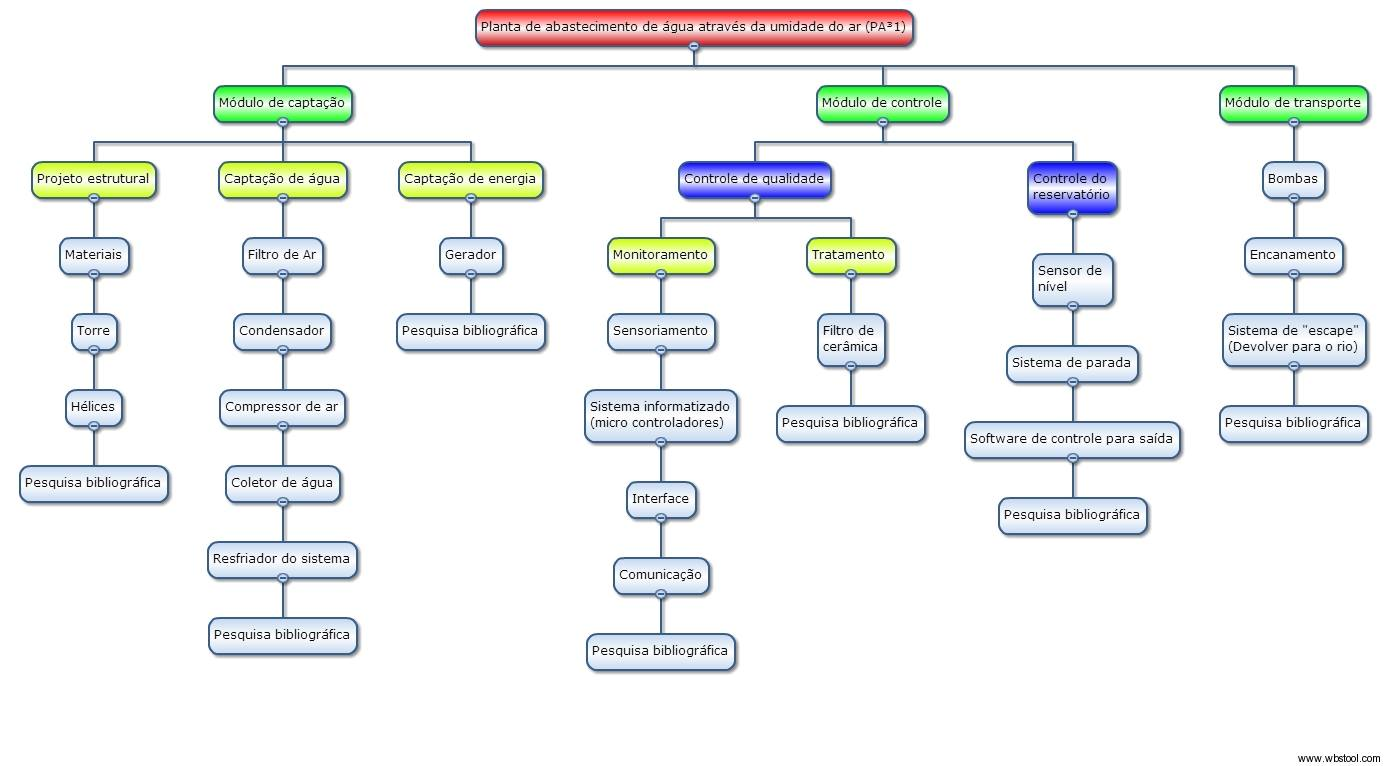
\includegraphics[scale=0.3]{editaveis/figuras/EAP}
\end{figure}
\FloatBarrier

\item Cronograma de marcos do projeto
O cronograma está descrito no item 5.3 da introdução.

\item Orçamento do projeto\\
Não há orçamento concreto para esse projeto em questão

\end{enumerate}
\section*{Metodologia}
A metodologia de desenvolvimento adotada neste projeto é uma adaptação de metodologias gerais de desenvolvimento
de produtos e serviços. Para a construção deste modelo de desenvolvimento foram selecionadas algumas técnicas de
projeto de produtos e serviços expostos em algumas obras de Slack (\citeyear{slack99}), Krajewski (\citeyear{krajewski96}) e Ramaswamy (\citeyear{ramaswamy96}).
Tais trabalhos descrevem formas de estabelecer etapas bem definidas para o desenvolvimento do projeto.\\
Como estrutura básica do projeto será adotada a seguinte metodologia, dividida em seis etapas:
\begin{figure}[h]
\centering
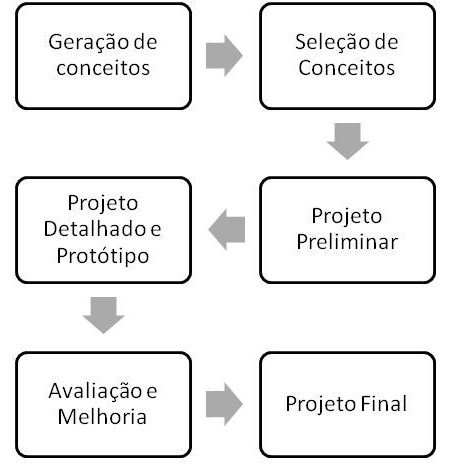
\includegraphics[scale=0.5]{editaveis/figuras/metodologia_de_desenvolvimento}
\end{figure}

\section*{Gestão de configuração}
A gestão de configuração foi o monitoramento das mudanças necessárias e viáveis para o progresso do projeto. As mudanças eram previamente colocadas em pauta na reunião e analisadas por todos, com o auxilio de dados e documentos sobre o porquê da mudança, depois de analisadas ela é aplicada e analisada novamente se a mesma não está em choque com as outras mudanças que  irão ser implementadas no mesmo momento.

\section*{Frequência de avaliação dos processos de gerenciamento do projeto}

Os processos de gerenciamento do projeto serão avaliados, primariamente, mensalmente, ou antes,
se surgirem problemas ou empecilhos para a continuação do projeto.

\section*{Alocação financeira para o gerenciamento do projeto.}

Não há dados de alocação financeira para o Gerenciamento de Projeto

\section*{Administração do plano de gerenciamento do projeto}
\begin{enumerate}
\item Responsável pelo plano:
\begin{itemize}
\item Rafael Abreu de Carvalho
\item Lais Rocha Carvalho
\end{itemize}
\item Frequência de atualização do plano de gerenciamento do projeto\\
	Terá no mínimo 1 atualização, o qual é a revisão programada ao termino desse plano. Poderá haver mais atualizações em menores escalas.

\end{enumerate}

\section*{Outros assuntos relacionados ao gerenciamento do projeto não previstos nesse plano}
Não há assuntos extras pertinentes ao plano de gerenciamento de Projeto

\section*{Documentos e planos auxiliares (anexos)}
\begin{itemize}
\item Plano de Gerenciamento das Comunicações
\item Plano de Gerenciamento de Escopo
\item Plano de Gerenciamento de Riscos
\item Plano de Gerenciamento de Recursos Humanos
\item Plano de Gerenciamento de Custos
\item Plano de Gerenciamento de Tempo
\item Plano de Gerenciamento de Qualidade
\item Plano de Gerenciamento das Aquisições
\item Cronograma do Projeto
\item EAP do projeto
\item Matriz de riscos do projeto


\end{itemize}

\section*{Documentos de referência}
\begin{itemize}
\item Declaração do Escopo Preliminar
\item Termo de abertura
\end{itemize}

\section*{Outras referências}
\begin{itemize}
\item PMBoK Guide 2004.
\end{itemize}

\section*{Assinaturas}
\begin{center}
Data: \rule{0.5cm}{0.1mm}/\rule{0.5cm}{0.1mm}/\rule{1cm}{0.1mm}     \\
\rule{13cm}{0.1mm}\\
ADRIANNY VIANA DE ARAÚJO AMORIM – GERENTE DE PROJETO\\

\end{center}
% \end{document}
  
\chapter{Plano de Gerenciamento das Comunicações}

  
\begin{center}
 {\large Plano de gerenciamento das Comunicações}\\[0.2cm]
 {Planta de abastecimento de água potável a partir da umidade do ar}\\
 \end{center}
 
 \section*{Histórico de Alterações}
\begin{table}[h]
\centering
\begin{tabular}{|c|c|p{6cm}|p{5cm}|}

Data & Versão & Descrição & Responsável\\
\hline                               
23/04/2015 & 0.0 & Criação do Plano de Gerenciamento das comunicações & Júlio César\\
\hline
24/04/2015 & 1.0 & Alteração: Incluído a descrição dos processos de gerenciamento das comunicações, eventos de comunicação, atas de reunião e administração dos plano de gerenciamento de comunicação. & 
Júlio César\\
\hline
\end{tabular}
\end{table}

\section*{Objetivo}
O objetivo desse plano é estabelecer um processo de gerenciamento das comunicações do projeto.

\section*{Descrição dos processos de gerenciamento das comunicações}
O processo de gerenciamento das comunicações é uma das áreas mais importantes para o gerenciamento de projetos, pois é a ligação entre as pessoas, as ideias e as informações. Além disso, a maioria dos problemas que ocorrem ao longo de um projeto é oriundo da falta de comunicação que gera o não entendimento entre as partes envolvidas cominando em um provável fracasso. O gerenciamento das comunicações do projeto inclui os processos necessários para garantir que as informações do projeto sejam geradas, coletadas, distribuídas, armazenadas, recuperadas e organizadas de forma eficiente. 

	As informações serão geradas através das diversas linhas de pesquisas, originadas em discussões e debates sobre o tema de interesse e serão tratadas em reuniões por todos da equipe. Estas informações também serão postadas, armazenadas e organizadas em nossos meios de comunicação virtual, que são realizados por meio da ferramenta de gerenciamento de projetos Trello, pela rede social Facebook e pelo serviço de armazenamento em nuvem gratuito Google Drive, além de ter todos os documentos salvos em um Pendrive.

\section*{Eventos de comunicação}
O projeto terá os seguintes eventos de comunicação:
\begin{table}[h]
\centering
\begin{tabular}{|p{5cm}|p{10cm}|}
Evento & Reunião Presencial\\
\hline
Objetivo & Verificar e informar o que foi feito, o que deverá ser feito e se há ou houve algum empecilho no decorrer das atividades\\
\hline
Metodologia & Encontros semanais.\\
\hline
Responsável & Adrianny Viana de Araújo Amorim\\
\hline
Envolvidos & Grupo I de Projeto Integrador 1\\
\hline
Data e Horário e/ou Freqüência & Segunda-feira e quarta-feira\\
\hline
Duração & 1 hora e 40 minutos\\
\hline
Local & Universidade de Brasília - Campus Gama

Segunda-feira: Sala I9

Quarta-feira: Sala I5\\
\hline
Outros & Reuniões realizadas em dias úteis

Verificação de presentes

Ausência mediante justificativa plausível\\
\hline

\end{tabular}
\end{table}

\section*{Atas de Reunião}
A ata de reunião é uma ferramenta que torna as reuniões mais eficientes e produtivas. Isto porque as decisões são anotadas e as atividades com seus respectivos responsáveis são acompanhadas. Informações essenciais são registadas na ata para que pessoas que não compareceram às reuniões possam saber do que se foi tratado, não havendo assim a necessidade de se perder tempo na próxima reunião repetindo fatos ocorridos. Essas informações também servem para facilitar a lembrança de temas pelos participantes, servir de bases para futuras discussões ou desentendimentos, forçar uma maior clareza sobre o que foi decidido, saber o que ainda falta fazer e poder se antecipar antes mesmo da reunião seguinte.

\section*{Relatórios do projeto}
Os principais relatórios a serem publicados no sistema de informações do projeto estão apresentados em anexo.

\section*{Ambiente técnico e estrutura de armazenamento e distribuição da informação (EPM)}
O ambiente técnico físico se concentra no Campus Gama da Universidade de Brasília, onde as discussões tratadas são registradas e armazenadas em computadores por meio de fotos e anotações e distribuídas virtualmente por meio de nossas ferramentas para que todos da equipe possam ter acesso e se manterem alinhados com o caminhar do projeto.

\section*{Administração do plano de gerenciamento das comunicações}
\begin{enumerate}

\item Responsável pelo plano:
\begin{itemize}

\item Júlio César Tavares Primo - Gerente de Comunicação
\item Vítor Ferreira Pacífico - Subgerente de Comunicação
\item Vitor Silva Ribeiro - Coordenador de Comunicação

\end{itemize}
\item Frequência de atualização do plano de gerenciamento das comunicações

	A frequência de atualização será realizada semanalmente de acordo com as alterações e acréscimos provindas das decisões das reuniões.
\end{enumerate}

\section*{Outros assuntos relacionados ao gerenciamento das comunicações do projeto não previstos nesse plano}
A comunicação interna entre os subgrupos designados para os específicos modelos de pesquisa

\section*{Assinaturas}
\begin{center}
Data: \rule{0.5cm}{0.1mm}/\rule{0.5cm}{0.1mm}/\rule{1cm}{0.1mm}     \\
\rule{13cm}{0.1mm}\\
ADRIANNY VIANA DE ARAÚJO AMORIM – GERENTE DE PROJETO\\
\rule{13cm}{0.1mm}\\
JÚLIO CÉSAR TAVARES PRIMO - GERENTE DE COMUNICAÇÃO


\end{center}
	  \pagebreak
  	\section{Relatórios de Comunicação}
  		%  \documentclass[12pt,openright,oneside,a4paper,brazil]{abntex2}
%  \usepackage[utf8]{inputenc}
%  \counterwithout{section}{section}
%  \counterwithout{figure}{chapter}
%  \counterwithout{table}{chapter}
%  \setlength{\parindent}{1.3cm}
%  \usepackage{indentfirst}
%  \setlength{\parskip}{0.2cm}
%  \usepackage[bottom=2cm,top=3cm,left=3cm,right=2cm]{geometry}
%  \usepackage{graphicx}
%  \graphicspath{{figuras/}}
%  \usepackage{placeins}
% 
% % opening
% % \title{}
% % \author{}
% 
%  \begin{document}
% 
% 
%  \textual
\begin{center}
{\large Relatório de comunicação 1}
\begin{table}[h]
\begin{tabular}{|p{6cm}|p{9cm}|}\hline
Relatorio & Relatório da Primeira Semana de reuniões; Reunião realizada dia 25/03/2015.\\ \hline
Objetivo & Definir Escopo do trabalho, amadurecer conceito da Teoria dos 5w 2h.\\ \hline
Informações & Na primeira semana, com reunião única foi definida o local pra implementação do projeto, as áreas de pesquisa a respeito do local assim como o “O que pesquisar” foi definido.\\ \hline
Responsável & Vitor Silva Ribeiro\\ \hline
Destinatários & Integrantes do Projeto, Professores Coordenadores.\\ \hline
Data e Horário e/ou Freqüência & Data: 25/03/2015 com horário de inicio 17h30min com termino as 18h00min\\ \hline
Local de Armazenagem & Relatório ficara armazenado facebook, no trelo, e no Google Doc.\\ \hline
Outros & O Relatório da comunicação será realizado semanalmente.\\ \hline

\end{tabular}
\end{table}

{\large Relatório de comunicação 2}
\begin{table}[h]
\begin{tabular}{|p{6cm}|p{9cm}|}\hline
Relatorio & Relatório da Segunda Semana de reuniões; Reunião realizada dia 01/04/2015.\\ \hline
Objetivo & A reunião tinha como objetivo explicar,detalhar e exemplificar a utilização da ferramenta de controle escolhida anteriormente (Trello).Separar duplas de pesquisa pra definição do tema (“O que”).\\ \hline
Informações & Na segunda semana, depois de definido os meios de comunicação, e os integrantes do grupo terem aderido ao mesmo, foi possível dar um passo a frente em relação ao tema, duplas de pesquisa foram formadas e um dos 5hs foi escolhido como ponto de partida (What).\\ \hline
Responsável & Vitor Silva Ribeiro\\ \hline
Destinatários & Integrantes do Projeto, Professores Coordenadores.\\ \hline
Data e Horário e/ou Freqüência & Data: 01/04/2015 com horário de inicio 17h42min com termino as 18h00min\\ \hline
Local de Armazenagem & Relatório ficara armazenado facebook, no trelo, e no Google Doc.\\ \hline
Outros & O Relatório da comunicação será realizado semanalmente.\\ \hline
\end{tabular}
\end{table}
\newpage

{\large Relatório de comunicação 3}
\begin{table}[h]
\begin{tabular}{|p{6cm}|p{9cm}|}\hline
Relatorio & Relatório da Terceira Semana de reuniões; Reunião realizada dia 06/04/2015\\ \hline
Objetivo & Apresentação das Pesquisas realizadas após a definição das duplas na ultima reunião. BrainStorm com foco  no escopo, tendo uma base sólida nas pesquisas.\\ \hline
Informações & Na terceira semana de reuniões, foram apresentadas idéias sobre dois locais de possível implementação do projeto, a plataforma de petróleo, e a cidade de Aracarí-Rn. As idéias foram implementas com pros e contras para cada ponto.\\ \hline
Responsável & Vitor Silva Ribeiro\\ \hline
Destinatários & Integrantes do Projeto, Professores Coordenadores.\\ \hline
Data e Horário e/ou Freqüência &Data: 06/04/2015 com horário de inicio 17h30min com termino as 18h00min\\ \hline
Local de Armazenagem & Relatório ficara armazenado facebook, no trelo, e no Google Doc.\\ \hline
Outros & O Relatório da comunicação será realizado semanalmente.\\ \hline
\end{tabular}
\end{table}

{\large Relatório de comunicação 4}
\begin{table}[h]
\begin{tabular}{|p{6cm}|p{9cm}|}\hline
Relatorio & Relatório da Terceira Semana de reuniões; Reuniões realizadas dias 13/04/2015 e 15/04/2015.\\ \hline
Objetivo & A quarta semana teve como principal objetivo definição do escopo, e a organização e separação/escolha, dos integrantes de acordo com as áreas de conhecimento do PMBok.\\ \hline
Informações & Na quarta semana, as discussões foram voltadas para a finalização do escopo, e a separação dos 9 grupos de acordo com o PMBok. Uma vez definidos, cada grupo ficou responsável pela entrega de seu próprio relatório.
Após as reuniões dessa semana ficaram claros os problemas iniciais. e as tecnologias empregadas no desenvolvimento do projeto foram filtradas, restando apenas uma.
Surgiu também uma base para a criação do FishBone.\\ \hline
Responsável & Vitor Silva Ribeiro\\ \hline
Destinatários & Integrantes do Projeto, Professores Coordenadores.\\ \hline
Data e Horário e/ou Freqüência & Data: 13/04/2015 com horário de inicio 17h30min com termino as 18h00min e 15/04/2015 com horário de inicio 16h13min com  termino as 17h50min\\ \hline
Local de Armazenagem & Relatório ficara armazenado facebook, no trelo, e no Google Doc.\\ \hline
Outros & O Relatório da comunicação será realizado semanalmente.\\ \hline
\end{tabular}
\end{table}
\FloatBarrier

{\large Relatório de comunicação 5}
\begin{table}[h]
\begin{tabular}{|p{6cm}|p{9cm}|}\hline
Relatório&Relatório da sexta semana de reuniões; Reunião realizada dia06/05/2015.\\ \hline
Objetivo&Revisar as pendências que ficaram para o ponto de controle 2 e observações feitas pelos orientadores.\\ \hline
Informações&	Explicação sobre o Scrum; Reunião dos gerentes e sub-gerentes com os orientadores;
Definição do Release Backlog (escopo do segundo ponto de controle);\\ \hline
Responsável	&Júlio César Tavares Primo\\ \hline
Destinatários&Integrantes do Projeto, Professores Coordenadores.\\ \hline
Data e Horário e/ou Freqüência& Data: 06/05/2015 com horário de inicio 16h30min com termino as 18h00min\\ \hline
Local de Armazenagem&Relatório ficará armazenado no Google Doc.\\ \hline
Outros&	O Relatório da comunicação será realizado semanalmente.\\ \hline
\end{tabular}
\end{table}
\FloatBarrier


{\large Relatório de comunicação 6}
\begin{table}[h]
\begin{tabular}{|p{6cm}|p{9cm}|}\hline
Relatório&	Relatório da sétima semana de reuniões; Reunião realizada dia 11/05/2015.\\ \hline
Objetivo	&Definir a quantidade de turbinas, suas disposições e demanda; Verificar resultados de pesquisa de cada frente.\\ \hline
Informações&	Discussão sobre as dimensões das turbinas e da área; Definições de atividades das frentes; Reunião dos professores com gerentes e subgerentes;\\ \hline
Responsável &	Júlio César Tavares Primo\\ \hline
Destinatários&Integrantes do Projeto, Professores Coordenadores.\\ \hline
Data e Horário e/ou Freqüência	& Data: 11/05/2015 com horário de inicio 16h10min com termino as 18h10min\\ \hline
Local de Armazenagem&Relatório ficará armazenado no Google Doc.\\ \hline
Outros&O Relatório da comunicação será realizado semanalmente.\\ \hline

\end{tabular}
\end{table}
\FloatBarrier

{\large Relatório de comunicação 7}
\begin{table}[h]
\begin{tabular}{|p{6cm}|p{9cm}|}\hline
Relatório&Relatório da oitava semana de reuniões; Reunião realizada dia18/05/2015.\\ \hline
Objetivo&Definição das dimensões de todos os componentes, preenchimento do formulário de acompanhamento de projeto (avaliação individual).\\ \hline
Informações &	Equipe de software terminando o levantamento de requisitos;
Todas as frentes reunidas para verificar os feitos e pendências;
Levantamento da viabilidade das torneiras (distribuição).\\ \hline
Responsável	&Júlio César Tavares Primo\\ \hline
Destinatários	&Integrantes do Projeto, Professores Coordenadores.\\ \hline
Data e Horário e/ou Freqüência	& Data: 18/05/2015 com horário de inicio 16h15min com termino as 17h55min\\ \hline
Local de Armazenagem&Relatório ficará armazenado no Google Doc.\\ \hline
Outros&O Relatório da comunicação será realizado semanalmente.\\ \hline
\end{tabular}
\end{table}
\FloatBarrier


{\large Relatório de comunicação 8}
\begin{table}[h]
\begin{tabular}{|p{6cm}|p{9cm}|}\hline
Relatório&Relatório da nona semana de reuniões; Reunião realizada dia20/05/2015.\\ \hline
Objetivo&Definiçãodas dimensões de todos os componentes;checagem de atividades feitas e pendências para o fechamento da sprint; \\ \hline
Informações&Ponto de controle dia 01/06 e 03/06;
Sprint finaliza dia 21/05;
Quarta a Sexta 12h as 14h monitores na mocap;
Livro de mecânica encontrado na biblioteca.\\ \hline
Responsável&Júlio César Tavares Primo\\ \hline
Destinatários&Integrantes do Projeto, Professores Coordenadores.\\ \hline
Data e Horário e/ou Freqüência&Data: 20/05/2015 com horário de inicio 16h05min com termino às 18h00min\\ \hline
Local de Armazenagem&Relatório ficará armazenado no Google Doc.\\ \hline
Outros&O Relatório da comunicação será realizado semanalmente.\\ \hline

\end{tabular}
\end{table}
\FloatBarrier

{\large Relatório de comunicação 9}
\begin{table}[h]
\begin{tabular}{|p{6cm}|p{9cm}|}\hline
Relatório&Relatório da décima semana de reuniões; Reunião realizada dia25/05/2015.\\ \hline
Objetivo&Definição da sprint 3;
Elaboração de relatório com feitos e pendências;
Preenchimento da auto-avaliação;\\ \hline
Informações	& Ponto de controle dia 01/06 e 03/06;
Entrega de relatório para quinta-feira (28/05);\\ \hline
Responsável&Júlio César Tavares Primo\\ \hline
Destinatários&Integrantes do Projeto, Professores Coordenadores.\\ \hline
Data e Horário e/ou Freqüência&Data: 25/05/2015 com horário de inicio 16h05min com termino às 18h05min\\ \hline
Local de Armazenagem&Relatório ficará armazenado no Google Doc.\\ \hline
Outros&O Relatório da comunicação será realizado semanalmente.\\ \hline
\end{tabular}
\end{table}
\FloatBarrier

{\large Relatório de comunicação 10}
\begin{table}[h]
\begin{tabular}{|p{6cm}|p{9cm}|}\hline
Relatório&Relatório da décima semana de reuniões; Reunião realizada dia27/05/2015.\\ \hline
Objetivo&Diagramas de fluxos da água e sua distribuição;
Discussão de pendências com o orientador;
Atualização dos planos, cronogramas e escopo;
Dimensionamento da torre;
Encerramento das atividades da sprint 3 de cada frente;
Preenchimento da auto-avaliação.\\ \hline
Informações&Requisitados as tensões das ventoinhas;
Especificações do gerador e do compressor pedidas;\\ \hline
Responsável&Júlio César Tavares Primo\\ \hline
Destinatários&Integrantes do Projeto, Professores Coordenadores.\\ \hline
Data e Horário e/ou Freqüência&Data: 27/05/2015 com horário de inicio 16h15min com termino às 17h50min\\ \hline
Local de Armazenagem&Relatório ficará armazenado no Google Doc.\\ \hline
Outros&O Relatório da comunicação será realizado semanalmente.\\ \hline
\end{tabular}
\end{table}
\FloatBarrier

{\large Relatório de comunicação 11}
\begin{table}[h]
\begin{tabular}{|p{6cm}|p{9cm}|}\hline
Relatório&Relatório da quinta Semana de reuniões; Reuniões realizadas dias 27/04/2015 e 29/04/2015.\\ \hline
Objetivo&Finalizar as tarefas referentes ao primeiro ponto de controle e dar continuidade ao projeto.\\ \hline
Informações&	Apresentação realizada para o dia 29/04.
Requisitos do sistema levantados pelo grupo de automotiva e aeroespacial.
Referencial teórico finalizado pelo pessoal de eletrônica.
Atualização no Latex por parte da gerência.\\ \hline
Responsável&Vitor Silva Ribeiro\\ \hline
Destinatários&Integrantes do Projeto, Professores Coordenadores.\\ \hline
Data e Horário e/ou Freqüência	&Data: 27/04/2015 com horário de inicio 16h30min com termino as 18h00min e 29/04/2015 com horário de inicio h min com termino as h min\\ \hline
Local de Armazenagem&Relatório ficara armazenado no Google Doc.\\ \hline
Outros	& O Relatório da comunicação será realizado semanalmente.\\ \hline
\end{tabular}
\end{table}
\FloatBarrier

\end{center}


% \end{document}

\chapter{Plano de Gerenciamento de Tempo}

  \documentclass[12pt,openright,oneside,a4paper,brazil]{abntex2}
\usepackage[utf8]{inputenc}
\counterwithout{section}{section}
\counterwithout{figure}{chapter}
\counterwithout{table}{chapter}
\setlength{\parindent}{1.3cm}
\usepackage{indentfirst}
\setlength{\parskip}{0.2cm}
\usepackage[bottom=2cm,top=3cm,left=3cm,right=2cm]{geometry}
\usepackage{graphicx}
\graphicspath{{figuras/}}
\usepackage{placeins}

%opening
\title{}
\author{}

\begin{document}


\textual
\begin{center}
 {\large Plano de gerenciamento de Tempo}\\[0.2cm]
 {Planta de abastecimento de água potável a partir da umidade do ar}\\
 \end{center}
 
 \section{Histórico de Alterações}
\begin{table}[h]
\centering
\begin{tabular}{|c|c|p{6cm}|p{5cm}|}

Data & Versão & Descrição & Responsável\\
\hline                               
22/04/2015 & 0.0 & Criação do plano de gerenciamento de tempo & Hugo Martins Ferreira\\
\hline
\end{tabular}
\end{table}

\section{Objetivo}
O objetivo desse plano é estabelecer um processo de gerenciamento do tempo do projeto.

Importância do plano de gerenciamento de tempo para o projeto:
O gerenciamento do tempo, quando feito de forma adequada, é fundamental para o desenvolvimento de qualquer projeto. Tendo isso em vista, esse plano de gerenciamento tem como objetivo garantir com que cada atividade relacionada ao desenvolvimento do projeto da Planta de Abastecimento de Água através da Umidade do Ar seja executada dentro de um intervalo de tempo determinado para cada uma delas para que assim seja assegurado o desenvolvimento do projeto sem  que haja atrasos.
	
\section{Descrição dos processos de gerenciamento do tempo}
Para assegurar o desenvolvimento do projeto dentro do prazo predeterminado foram definidos processos de gerenciamento que serão seguidos: gerenciar, desenvolver e controlar o cronograma, definição das atividades, sequenciar as atividades, estimar as durações das atividades e estimar os recursos das atividades.
\begin{itemize}
\item Gerenciar, desenvolver e controlar o cronograma:\\
Esses processos relacionados ao cronograma envolvem a sua criação definindo as atividades que estão envolvidas com o desenvolvimento do projeto. Cada uma dessas atividades possui uma ordem de execução, pois algumas atividades estão ligadas à outras e por isso precisam seguir o seu tempo de execução para não atrasar nenhum passo no desenvolvimento do projeto. Para assegurar que esses processos estão sendo seguidos da maneira que deve ser, existe um membro (ou um grupo de membros) da equipe do projeto que é responsável pelo controle do cronograma.
\item Definição das atividades:\\
Esse processo envolve a identificação das atividades para o desenvolvimento do projeto e, além de identificar as atividades, esse processo delega responsáveis por cada uma delas. Cada uma dessas atividades e os seus devidos responsáveis devem ser registrados no cronograma.
\item Sequenciar as atividades:\\
Esse processo determina as datas e a ordem das entregas de cada uma das atividades. Como já foi dito, essa ordem é importante, pois algumas atividades dependem de outras.
\item Estimar as durações das atividades:\\
Esse processo determina o tempo de execução de cada atividade, pois é necessário para seguir a ordem da sequência das entregas das atividades para que não haja atraso no cronograma.
\item Estimar os recursos das atividades:\\
Esse processo determina quais são os recursos necessários para o desenvolvimento de cada atividade. Esses recursos podem ser recursos humanos, materiais, equipamentos, suprimentos ou informações de outras atividades.
\end{itemize}

\section{Priorização das mudanças nos prazos}
Para que não haja muita mudança no planejamento de execução do projeto, dificilmente haverá mudança nos prazos de entrega das atividades. Só poderá haver mudanças caso ocorra um aumento no prazo de entrega do projeto. De resto, o máximo que pode acontecer é uma antecipação no início de uma atividade, fazendo com isso que a equipe responsável pela mesma tenha um prazo maior na execução da mesma. Para isso acontecer, a atividade anterior, caso ela seja insumo para esta atividade, precisa ter sido concluída antes do seu período máximo de execução.

\section{Sistema de Controle de Mudanças de Prazos (SCMP)}
As mudanças de prazos no projeto deverão ser previamente autorizadas pela equipe de gerência. As mudanças deverão ser comunicadas previamente e deverão seguir o prazo limite de tempo que será estabelecimento anteriormente a cada atividade. Haverá um registro de mudanças que será atualizado sempre que houver alguma mudança no prazo de entrega de atividades. O registro de mudanças no projeto deverá ser entregue a todos os interessados no projeto, pois pode influenciar diretamente no tempo, nos custos e nos riscos do mesmo. Desta forma, as aprovações das mudanças de prazo deverão ser revisadas pelas equipes de gerenciamento de custo, tempo e riscos. As mudanças poderão ser realizadas sempre que houver uma reserva de tempo. Esta reserva deve ser utilizada para o término de atividades inacabadas ou para atividades acrescentadas que seguirem às especificações das equipes de gerenciamento.

\section{Mecanismo adotado para o conciliamento de recursos}
Sempre que uma atividade for definida, dever-se-á realizar uma alocação de recursos designados para suprir a demanda daquela atividade. Caso haja reserva de tempo ou custos, estes recursos serão alocados para alguma atividade. O mecanismo de escolha desta atividade será seguir a ordem de importância da mesma para o projeto, ou seja, a atividade mais importante para o desenvolvimento do projeto alocará os recursos extras. 

\section{Reserva de tempo do projeto}
O projeto contará com uma reserva de tempo sempre que for extremamente necessário. Porém, esta reserva de tempo somente existirá quando aprovada pelo conselheiro do grupo de projeto. A reserva de tempo também pode existir devido á alguma mudança na alocação de tempo para o desenvolvimento das atividades.

\section{Frequência de avaliação dos prazos do projeto}
A avaliação dos prazos do projeto será realizada semanalmente.

\section{Alocação financeira para o gerenciamento do tempo}
A alocação de recursos financeiros pode ser modificada por alguma mudança realizada pela equipe de gerenciamento de tempo. Desta forma, a equipe de gerenciamento de custos deve estar sempre informada das mudanças realizadas pela equipe de gerenciamento do tempo.

\section{Administração do plano de gerenciamento do tempo}
\begin{enumerate}

\item Responsável pelo plano:
\begin{itemize}
\item Hugo Martins Ferreira
\item Ana Paula Chavier Rodrigues
\end{itemize}
\item Frequência de atualização do plano de gerenciamento do tempo

A atualização do plano de gerenciamento do projeto será realizada mensalmente.
\end{enumerate}
\section{Assinaturas}
\begin{center}
Data: \rule{0.5cm}{0.1mm}/\rule{0.5cm}{0.1mm}/\rule{1cm}{0.1mm}     \\
\rule{13cm}{0.1mm}\\
ADRIANNY VIANA DE ARAÚJO AMORIM – GERENTE DE PROJETO\\
\rule{13cm}{0.1mm}\\
HUGO MARTINS FERREIRA- GERENTE DE TEMPO

\end{center}
\end{document}

\chapter{Plano de Gerenciamento de Qualidade}

  \documentclass[12pt,openright,oneside,a4paper,brazil]{abntex2}
\usepackage[utf8]{inputenc}
\counterwithout{section}{section}
\counterwithout{figure}{chapter}
\counterwithout{table}{chapter}
\setlength{\parindent}{1.3cm}
\usepackage{indentfirst}
\setlength{\parskip}{0.2cm}
\usepackage[bottom=2cm,top=3cm,left=3cm,right=2cm]{geometry}
\usepackage{graphicx}
\graphicspath{{figuras/}}
\usepackage{placeins}

%opening
\title{}
\author{}

\begin{document}


\textual
\begin{center}
 {\large Plano de gerenciamento de Qualidade}\\[0.2cm]
 {Planta de abastecimento de água potável a partir da umidade do ar}\\
 \end{center}
 
 \section{Histórico de Alterações}
\begin{table}[h]
\centering
\begin{tabular}{|c|c|p{6cm}|p{5cm}|}

Data & Versão & Descrição & Responsável\\
\hline                               
19/04/2015 & 0.0 & Criação do Plano de Gerenciamento de Qualidade & Alexandre T. Kryonidis, André Luis, Matheus Jericó\\
\hline
20/04/2015 & 1.0 & Revisão do Plano & Alexandre K., André Luis.\\
\hline
\end{tabular}
\end{table}

\section{Objetivo}
  O objetivo desse plano é estabelecer um processo de gerenciamento e controle da qualidade do projeto.
  
\section{Descrição dos processos de gerenciamento da qualidade}
 A qualidade de um projeto está relacionada, principalmente, com o cumprimento dos requisitos levantados, ou seja, satisfaz os objetivos a que o projeto se propôs a solucionar. Dessa forma pretende-se gerenciar a qualidade do projeto da seguinte maneira:
 \begin{itemize}

\item As alterações nos requisitos de qualidade previstos para o sistema devem passar por uma avaliação do sistema de controle de mudanças da qualidade.
\item Todas as reclamações provenientes dos stakeholders serão avalidadas e, ao corrigi-las, deverão ser tratadas como medidas corretivas no plano de gerenciamento da qualidade.
\item Todos os produtos ou entregas que não cumprem obedecem a declaração de escopo deverão ser tratadas como medidas corretivas no plano de gerenciamento de qualidade.
\item As solicitações de mudanças devem ser documentadas de acordo com o plano de comunicações do projeto.	
 \end{itemize}
 
 \section{Priorização das mudanças nos quesitos de qualidade e respostas}
 \begin{itemize}
 \item Prioridade Alta
 
 Mudanças de alta prioridade causam um grande impacto no projeto e deverão ser tratadas em caráter de urgência, pelo gerente do Projeto, em conjunto com algum membro da equipe de qualidade. Essas mudanças devem ser abordadas durante as  reuniões de grupos apesar delas serem independentes das reuniões de controle, devido ao seu grau de importância. 
 
 \item Prioridade Média
 
 Mudanças de média prioridade envolvem um impacto que requer ação rápida do Gerente de Projeto, também em conjunto com a equipe de qualidade. Podem ser tomadas antes das reuniões de controle, mas também é possivel esperar um pequeno prazo para serem avaliadas por um número maior de “steakholders”. Os resultados dessa mudança também devem ser debatidos nas reuniões.

\item Prioridade Baixa

	Mudanças de prioridade Baixa não acarretam alterações significativas na elaboração do projeto e, portanto, não é requerida uma ação imediata, está dentro da autonomia de qualquer integrante da gerencia do Projeto
 \end{itemize}
 
 \section{Sistema de controle de mudanças da qualidade}
 As realizações do controle de qualidade das entradas, que passaram por solicitações de mudanças devem ser verificadas, podendo ocorrer modificações como reparo de defeitos, revisão dos métodos de trabalho e revisão do cronograma. Nas saídas, os itens alterados ou reparados são inspecionados e serão aceitos ou rejeitados antes do fornecimento. Os rejeitados podem exigir retrabalho.
 \begin{figure}[h]
 \begin{center}

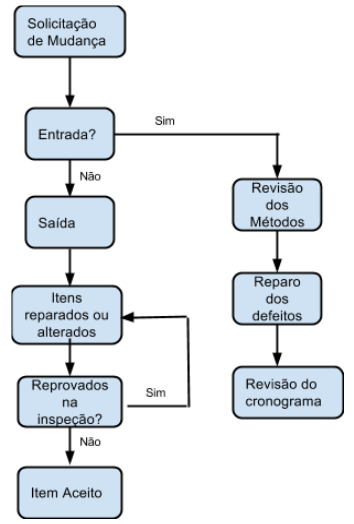
\includegraphics[scale=0.6]{mudanca}
\label{Mudanca}
 \end{center}
 \end{figure}
 \FloatBarrier
 
 \section{Frequência de avaliação dos requisitos de qualidade do projeto}
 Os requisitos de qualidade serão avaliados e, caso necessário, atualizados de duas em duas semanas. Os resultados obtidos a partir das análises relacionados a qualidade do projeto serão apresentados nas reuniões presenciais do grupo.

\section{Alocação financeira das mudanças nos requisitos de qualidade}
Todas as mudanças a serem efetuadas devem entar dentro do previsto pela equipe de gerenciamento de custo, qualquer alteração que impacte no orçamento do projeto, será discutida com os reponsáveis pelo custo. Como não temos patrocinadores nesse momento, não teremos formas de adquirir novos recursos com facilidade, por isso, gastos adicionais devem ser evidados. Porém, se esse gasto adicinal trouxer beneficios consideráveis para o projeto não deverá ser descartado. Qualquer necessidade de avaliação de custos será atribuida a equipe de gerenciamento de custo, ou estará sujeita a  análise e aprovação pela mesma.

\section{Administração do plano de gerenciamento da qualidade}
\begin{enumerate}
\item Responsável pelo plano:
\begin{itemize}
\item Alexandre Torres Kryonidis - Gerente de qualidade.
\item André Luis - suplente do responsável pelo plano de gerenciamento de qualidade.
\end{itemize}
\item	Freqüência de atualização do plano de gerenciamento da qualidade

O plano de qualidade será avaliado quinzenalmente e, caso necessário, será atualizado após essas avaliações. Qualquer necessidade de alteração no plano antes desse periodo, deverá ser tratado segundo os procedimentos tratados no item IX (Outros assuntos relacionados ao gerenciamento da qualidade do projeto não previstos neste plano)
\end{enumerate}

\section{Outros assuntos relacionados ao gerenciamento da qualidade do projeto não previstos nesse plano}
Qualquer solicitação que não se enquadrem nos preceitos deste plano deverão ser abordados nas reuniões semanais de acompanhamento do projeto, desse forma, serão dados os devidos encaminhamentos. Após as aprovações, o plano de gerenciamento será atualizado com os devidos registros.
\section{Assinaturas}
\begin{center}
Data: \rule{0.5cm}{0.1mm}/\rule{0.5cm}{0.1mm}/\rule{1cm}{0.1mm}     \\
\rule{13cm}{0.1mm}\\
ADRIANNY VIANA DE ARAÚJO AMORIM – GERENTE DE PROJETO\\
\rule{13cm}{0.1mm}\\
ALEXANDRE TORRES KRYONIDIS - GERENTE DE QUALIDADE

\end{center}
\end{document}
  
\chapter{Plano de Gerenciamento de Aquisições}

  % \documentclass[12pt,openright,oneside,a4paper,brazil]{abntex2}
% \usepackage[utf8]{inputenc}
% \counterwithout{section}{section}
% \counterwithout{figure}{chapter}
% \counterwithout{table}{chapter}
% \setlength{\parindent}{1.3cm}
% \usepackage{indentfirst}
% \setlength{\parskip}{0.2cm}
% \usepackage[bottom=2cm,top=3cm,left=3cm,right=2cm]{geometry}
% \usepackage{graphicx}
% \graphicspath{{figuras/}}
% \usepackage{placeins}

% opening
% \title{}
% \author{}

% \begin{document}


% \textual
\begin{center}
 {\large Plano de gerenciamento das Aquisições}\\[0.2cm]
 {Planta de abastecimento de água potável a partir da umidade do ar}\\
 \end{center}
 
 \section{Histórico de Alterações}
\begin{table}[h]
\centering
\begin{tabular}{|c|c|p{6cm}|p{5cm}|}

Data & Versão & Descrição & Responsável\\
\hline                               
19/04/2015 & 0.0 & Criação do Plano de Gerenciamento das aquisições e o preenchimento da descrição dos processos e os tipos de contratos. & Gustavo Pereira\\
\hline
20/04/2015 & 1.0 & Alterações do tópico III e o preenchimento dos tópicos IV, V, VI, VII, IX e X. & Gustavo Pereira, Yan Watanabe, Brenda Tagna\\
\hline
22/04/2015 & 2.0 & Atualização e retirada de alguns textos nos itens III e IV. Reorganização dos critérios de avaliação do item VI. & Gustavo Pereira, Yan Watanabe, Brenda Tagna\\
\hline
23/04/2015 & 2.0 & Preenchimento do item VIII de acordo com os requisitos inicias do projeto. & Gustavo Pereira, Yan Watanabe, Brenda Tagna\\
\hline
\end{tabular}
\end{table}

\section{Objetivo}
  O objetivo desse plano é estabelecer um processo de gerenciamento das aquisições do projeto.
  
\section{Descrição dos processos de gerenciamento das aquisições}
  Esse processo será desenvolvido por Gustavo Pereira, Yan Watanabe e Brenda Tagna. Esse plano de aquisição tem como objetivo listar todos os serviços e produtos a serem adquiridos por meio de contratos. 
A escolha de um determinado fornecedor ou prestador de serviço, será feita de uma forma em que possamos analisar itens considerados de extrema importância para um acordo contratual, como os listados no item V e VI desse plano. A partir dessa análise poderá ser feita uma escolha que melhor atenda aos requisitos do projeto. 
Todas as aquisições deverão seguir um padrão ético, sempre buscando a melhor escolha para o projeto, sem que haja benefício ilícito. 

   
\section{Gerenciamento e tipos de contratos}
Para o projeto em questão, serão usados principalmente contratos de Preço Fixo, uma vez que esse tipo de contrato é o mais recomendado para projetos de escopo bem detalhado, como esse. 
Existem algumas variações do contrato de Preço Fixo:
\begin{itemize}

\item PFG: Preço fixo garantido
\item PFRI: PF + Remuneração de Incentivo (ex: prêmio para entrega no prazo, excelência no serviço prestado, etc)
\item PFAEP: PF com Ajuste Econômico do Preço
\end{itemize}

\section{Critérios de avaliação de cotações e propostas}
\begin{itemize}
\item Preço;
\item Boa referência de serviços prestados
\item Certificaçao de produtos e serviços prestados
\item Forma de pagamento
\end{itemize}

\section{Avaliação de fornecedores}
\begin{itemize}
\item Adequação aos requisitos do projeto
\item Preço
\item Prazo
\item Assistência Técnica pré (consultoria) e pós compra
\item Forma de pagamento
\item Boa referência de serviços prestados
\item Qualidade
\item Garantia do produto ou serviços
\item Certificação de produtos e serviços prestados
\end{itemize}

\section{Frequência de avaliação dos processos de aquisição}
A frequência de verificação dependerá de cada contrato. Em um período de duas semanas antes do término do mesmo, será analisada a necessidade de renovação ou encerramento, levando em consideração o cumprimento (ou não) das cláusulas do contrato.

\section{Alocação financeira para o gerenciamento das aquisições}
Para a alocação financeira  inicial do projeto, será necessário adquirir os seguintes itens:
\begin{table}[h]
\centering
\begin{tabular}{|p{7cm}|c|p{2cm}|p{2.5cm}|}
Itens & Tipo de Contrato & Quantidade & Valor\\
\hline
Aquisição de computadores & Preço Fixo	& 25 & R\$ 30.000,00 \\
\hline
Aquisição do Pacote Office 365 Business Premium (Semestral)	& Preço Fixo & 25 & R\$ 7.350,00\\
\hline
Impressora Multifuncional & Preço Fixo & 1 & R\$ 3.500,00\\
\hline
Plano de Internet (Semestral) & Preço Fixo & 1 & R\$ 720,00\\
\hline
 & & Total & R\$ 41.570,00
\end{tabular}
\end{table}

\section{Administração do plano de gerenciamento das aquisições}
\begin{enumerate}
\item Responsável pelo plano:
\begin{itemize}
\item Yan Watanabe Martins – gerente de Aquisições
\item Gustavo Pereira – suplente do responsável direto pelo plano de gerenciamento de Aquisições
\end{itemize}
\item Freqüência de atualização do plano de gerenciamento das aquisições:
O Plano de Gerenciamento de Aquisições será revisado em cada reunião. As reuniões ocorrem pelo menos duas vezes por semana. Tal plano poderá ser modificado (ou não) levando em consideração as determinações e avaliações dos resultados de cada membro da equipe. 
\end{enumerate}

\section{Outros assuntos relacionados ao gerenciamento das aquisições do projeto não previstos nesse plano}
Todas as mudanças referentes ao Plano de Gerenciamento de Aquisições deverão ser apresentadas e discutidas em reunião, sendo a equipe de Aquisição a responsável por tal avaliação. A responsabilidade de possíveis mudanças no quadro pessoal da equipe fica direcionada aos gerentes de projeto.

\section{Assinaturas}
\begin{center}
Data: \rule{0.5cm}{0.1mm}/\rule{0.5cm}{0.1mm}/\rule{1cm}{0.1mm}     \\
\rule{13cm}{0.1mm}\\
ADRIANNY VIANA DE ARAÚJO AMORIM – GERENTE DE PROJETO\\
\rule{13cm}{0.1mm}\\
YAN WATANABE - GERENTE DE AQUISIÇÕES

\end{center}
% \end{document}

\chapter{Plano de Gerenciamento de Custos}

  % \documentclass[12pt,openright,oneside,a4paper,brazil]{abntex2}
% \usepackage[utf8]{inputenc}
% \counterwithout{section}{section}
% \counterwithout{figure}{chapter}
% \counterwithout{table}{chapter}
% \setlength{\parindent}{1.3cm}
% \usepackage{indentfirst}
% \setlength{\parskip}{0.2cm}
% \usepackage[bottom=2cm,top=3cm,left=3cm,right=2cm]{geometry}
% \usepackage{graphicx}
% \graphicspath{{figuras/}}
% \usepackage{placeins}

% opening
% \title{}
% \author{}

% \begin{document}


% \textual
\begin{center}
 {\large Plano de gerenciamento de Custos}\\[0.2cm]
 {Planta de abastecimento de água potável a partir da umidade do ar}\\
 \end{center}
 
 \section*{Histórico de Alterações}
\begin{table}[h]
\centering
\begin{tabular}{|c|c|p{6cm}|p{5cm}|}

Data & Versão & Descrição & Responsável\\
\hline                               
17/04/2015 & 0.0 & Criação deste documento para descrever todo planejamento de custo do projeto. & Guilherme Matias, João Gabriel, Pedro Kelvin.\\ \hline
\end{tabular}
\end{table}

\section*{Objetivo}

O objetivo desse plano é estabelecer um processo de gerenciamento de custos do projeto
  
\section*{Descrição dos processos de gerenciamento de custo}

A gerência do custo do projeto agrega os processos que envolvem planejamento, estimativa, orçamento e controle de custos que serão necessários para a conclusão do projeto a partir de uma previsão orçamentária. Onde a estimativa de custo desenvolve uma aproximação dos gastos com recursos necessários para a elaboração do projeto, quantoao orçamento, agregar os custos estimados de atividades ou de pacotes individuais de trabalho para estabeleceru ma base de custo, e o controle influência nos fatores que geram uma variação de custo e controlar as mudanças de orçamento de projeto. O gerenciamento de custos será analisado desde a fase de iniciação do projeto até o seu encerramento. O processo de gerenciamento será feito através de dados queiram dizer se a relação custo/benefício está sendo viável ou não para o projeto, analisando o custos de: tecnologia utilizada para a condensação do ar, estrutura da planta, tempo de retorno do valor investido. Será usado a técnica do PMBOK para gerir a estimativa de custo e orçamento do projeto. Serão analisados para saber em que vai influenciar do decorrer do projeto, e então corrigí-lo.

\section*{Frequência de avaliação do orçamento do projeto e das reservas gerenciais}   

O orçamento será avaliado semanalmente, durante as reuniões da equipe de custos. A exposição dos resultados para o resto da equipe será feita quinzenalmente, durante as reuniões gerais.

\section*{Reservas gerenciais}

Não se aplica.

\section*{Autonomias}

Não se aplica.

\section*{Alocação financeira das mudanças no orçamento}

As mudanças de caráter corretivo podem ser alocadas dentro das reservas gerenciais do projeto, desde que dentro da alçada do gerente de projeto.

\section*{Administração do plano de gerenciamento de custos}
\begin{itemize}

\item Responsável pelo plano:

\begin{enumerate}
\item João Gabriel da Silva Souza – Gerente de planejamento de custos
\item Guilherme Matias – Coordenador do planejamento de custos
\end{enumerate}

\item Freqüência de atualização do plano de gerenciamento de custos\\

A frequência de atualização será realizada duas vezes por semana, de acordo com as exigências apresentadas.
\end{itemize}

\section*{Outros assuntos relacionados ao gerenciamento de custos do projeto não previstos nesse plano}
Todas as alterações não previstas neste plano devem ser submetidas à reunião para aprovação. Imediatamente após sua aprovação devem ser atualizadas no plano de gerenciamento dos custos com seu devido registro de atualização.

\section*{Assinaturas}
\begin{center}
Data: \rule{0.5cm}{0.1mm}/\rule{0.5cm}{0.1mm}/\rule{1cm}{0.1mm}     \\
\rule{13cm}{0.1mm}\\
ADRIANNY VIANA DE ARAÚJO AMORIM – GERENTE DE PROJETO\\
\rule{13cm}{0.1mm}\\
JOÃO GABRIEL DA SILVA SOUZA - GERENTE DE CUSTO
\end{center}
% \end{document}

\chapter{Plano de Gerenciamento de Escopo}

 \documentclass[12pt,openright,oneside,a4paper,brazil]{abntex2}
\usepackage[utf8]{inputenc}
\counterwithout{section}{section}
\counterwithout{figure}{chapter}
\counterwithout{table}{chapter}
\setlength{\parindent}{1.3cm}
\usepackage{indentfirst}
\setlength{\parskip}{0.2cm}
\usepackage[bottom=2cm,top=3cm,left=3cm,right=2cm]{geometry}
\usepackage{graphicx}
\graphicspath{{figuras/}}
\usepackage{placeins}

%opening
\title{}
\author{}

\begin{document}
\textual
\begin{center}
 {\large Plano de gerenciamento de Tempo}\\[0.2cm]
 {Planta de abastecimento de água potável a partir da umidade do ar}\\
 \end{center}
 
 \section{Histórico de Alterações}
\begin{table}[h]
\centering
\begin{tabular}{|c|c|p{6cm}|p{5cm}|}

Data & Versão & Descrição & Responsável\\
\hline                               
22/04/2015 & 0.0 & Criação do plano de gerenciamento de escopo & Rafael Abreu de Carvalho, Filippe Leal, Ítalo Paiva Batista. \\
\hline
\end{tabular}
\end{table}

\section{Objetivo}
O objetivo desse plano é estabelecer um processo de gerenciamento do escopo do projeto.

\section{Descrição dos processos de gerenciamento de escopo}
O escopo produzido para a realização do projeto foi baseado em um documento padrão do projeto proposto, no qual era apresentados a ideia principal e os requisitos que o produto final do projeto deveria suprir ao final do processo, também foi feita uma pesquisa completa sobre as características região escolhida, sobre as características da população residente no local e sobre as tecnologias disponíveis no mercado, o qual suprirá os requisitos apresentados anteriormente. Durante a elaboração do escopo foram criadas uma EAP (estrutura analítica de processo) e uma análise de riscos por meio de uma estrutura Fishbone, documentos primordiais para a decisão do escopo em questão.

As regras para mudanças de escopo foram definidas em cima de características que visam respeitar o espaço determinado no inicio, respeitar os requisito determinados pela proposta inicial do projeto, respeitar as características do local, respeitar a ideia de custo e eficiência e respeitar as necessidades da população local. Tais mudanças deverão ser embasadas por pesquisa cientificas concreta e com alerta prévio.

\section{Priorização das mudanças do escopo e respostas}
As mudanças serão priorizadas para suprir as alterações e consequências que refletiram no quesito de requisitos primordiais do projeto, depois dessa analise os outros quesitos de mudança serão analisados e efetivados no escopo.

\section{Gerenciamento das Configurações (GC)}
\begin{figure}[!ht]
\centering
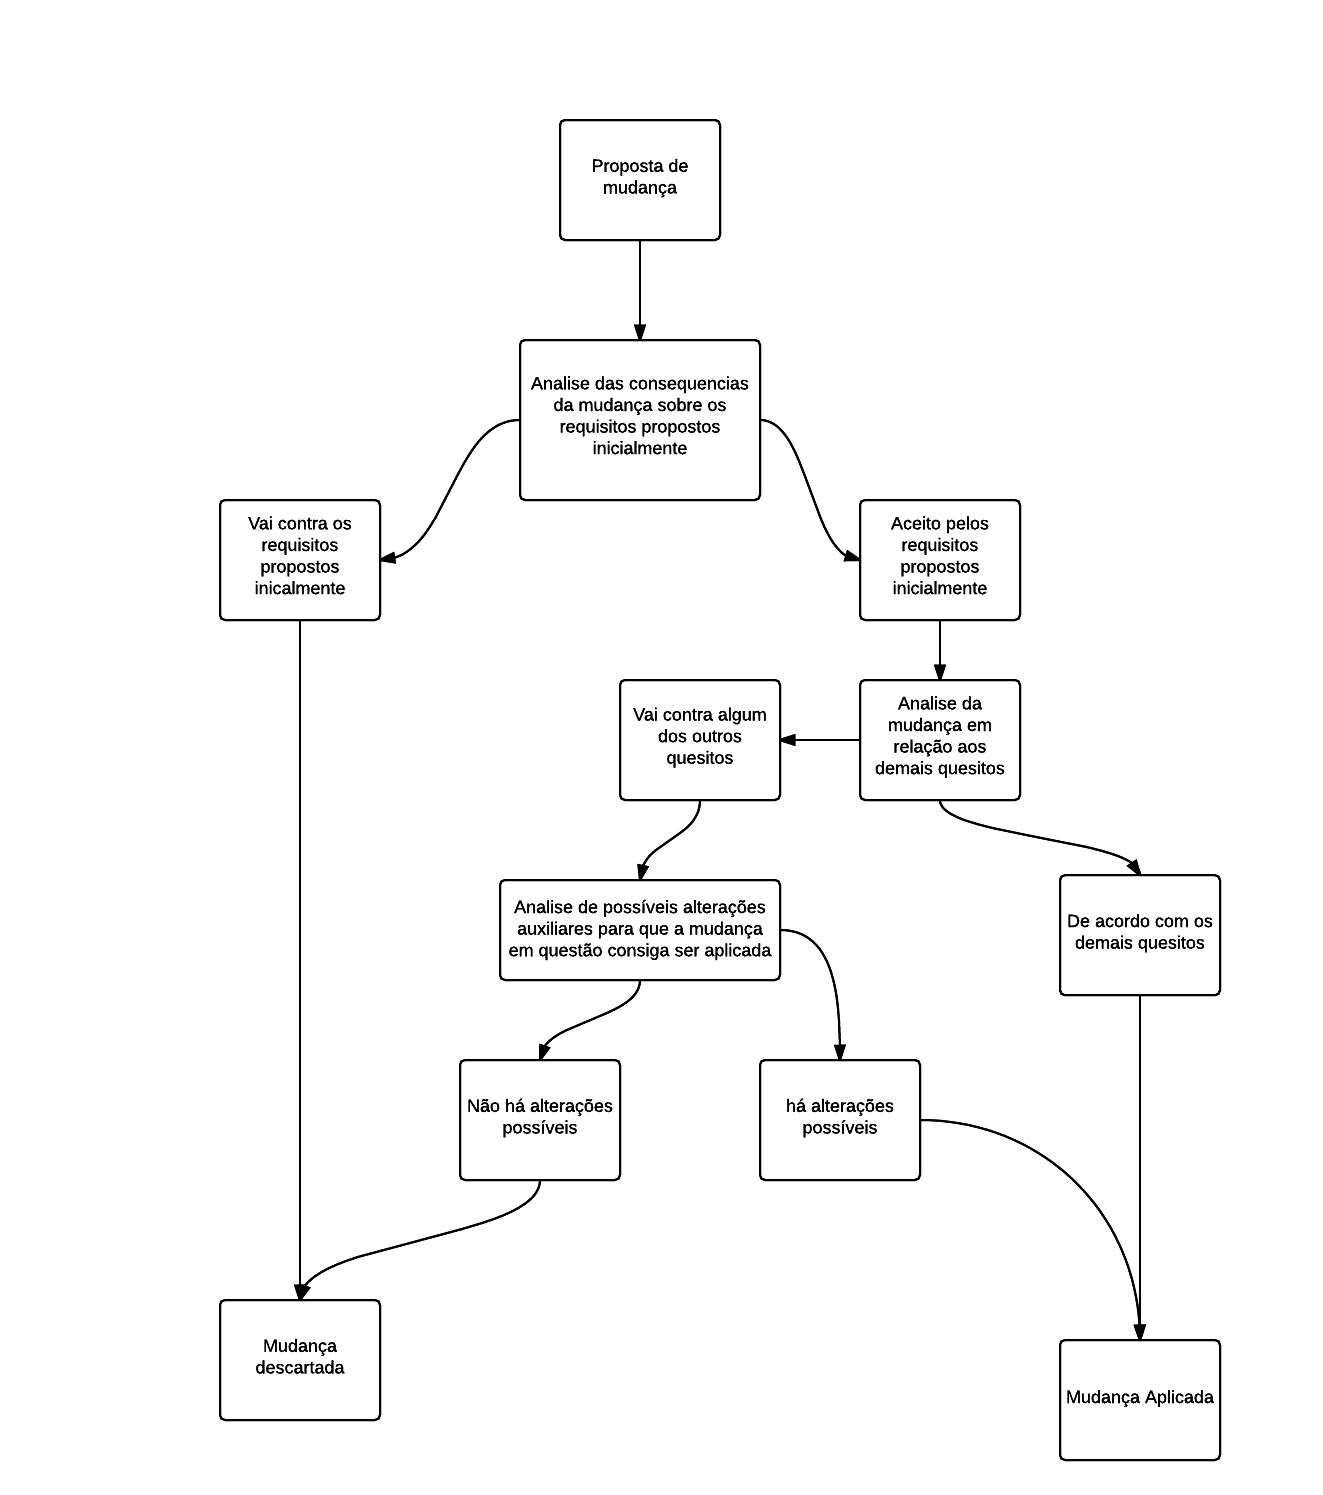
\includegraphics[scale=0.5]{configuracoes}
\label{Rotulo}
\end{figure}
\FloatBarrier

\section{Frequência de avaliação do escopo do projeto.}
O escopo final não sofreu grandes mudanças, devido a fato do mesmo ter surgido após muitas pesquisas e reuniões de grupo, então a frequência de mudanças foi praticamente nula.

\section{Alocação financeira das mudanças de escopo.}
Não houve mudanças impactantes na área de custos do projeto depois da finalização do escopo. Caso houve tais mudanças as mesmas seriam feita de forma a balancear o custo de uma área com os das outras áreas priorizando a parte de tecnologia necessária para que o projeto funcione.

\section{Administração do plano de gerenciamento de escopo:}
\begin{enumerate}

\item Responsável pelo plano:
\begin{itemize}
\item Rafael Abreu de Carvalho
\item Ítalo Paiva Batista

\end{itemize}

\item Freqüência de atualização do plano de gerenciamento de escopo
Como não houve mudanças no escopo depois de definido o documento final, a frequência de atualização foi nula.
\end{enumerate}

\section{Outros assuntos relacionados ao gerenciamento do escopo do projeto não previstos nesse plano}
A única mudança feita foi uma revisão para deixa-lo mais claro e objetivo para o escopo ficar melhor de ser entendido

\section{Assinaturas}
\begin{center}
Data: \rule{0.5cm}{0.1mm}/\rule{0.5cm}{0.1mm}/\rule{1cm}{0.1mm}     \\
\rule{13cm}{0.1mm}\\
ADRIANNY VIANA DE ARAÚJO AMORIM – GERENTE DE PROJETO\\
\rule{13cm}{0.1mm}\\
ÍTALO PAIVA BATISTA - GERENTE DE TEMPO

\end{center}
\end{document}

\chapter{Plano de Gerenciamento de Recursos Humanos}

  \documentclass[12pt,openright,oneside,a4paper,brazil]{abntex2}
\usepackage[utf8]{inputenc}
\counterwithout{section}{section}
\counterwithout{figure}{chapter}
\counterwithout{table}{chapter}
\setlength{\parindent}{1.3cm}
\usepackage{indentfirst}
\setlength{\parskip}{0.2cm}
\usepackage[bottom=2cm,top=3cm,left=3cm,right=2cm]{geometry}
\usepackage{graphicx}
\graphicspath{{figuras/}}
\usepackage{placeins}

%opening
\title{}
\author{}

\begin{document}


\textual
\begin{center}
 {\large Plano de gerenciamento dos Recursos Humanos}\\[0.2cm]
 {Planta de abastecimento de água potável a partir da umidade do ar}\\
 \end{center}
 
 \section{Histórico de Alterações}
\begin{table}[h]
\centering
\begin{tabular}{|c|c|p{7cm}|c|}

Data & Versão & Descrição & Responsável\\
\hline                               
19/04/2015 & 0.0 & Criação do plano de recursos humanos e suas especificações. & Amanda Leite de Castro\\
\hline
\end{tabular}
\end{table}

\section{Objetivo}
  O objetivo desse plano é estabelecer um processo de gerenciamento dos recursos humanos do projeto.
  
  \section{Perfil dos recursos humanos}
  \begin{itemize}
   \item Gerente de Projeto – Adrianny Viana de Araújo Amorim: responsável pelo projeto; realizar a gestão da mudança, escopo, custo, qualidade e os recursos que serão compartilhados entre os vários setores do projeto; selecionar e adaptar os processos de gerenciamento de projetos mais apropriados para a realidade da gerência, na medida da necessidade; dirigir e liderar a equipe, almejando a realização dos objetivos e metas; acompanhar a maturidade da equipe em gerenciamento de projetos, identificando necessidades de orientação e treinamentos; aprovar o plano de cada parte do projeto e autoriza sua execução; definir documentos padrões, base de dados e ferramentas; convocar e coordenar reuniões do projeto; administrar conflitos; definir o escopo do produto.
   \item Gerente setorial: responsável por gerenciar as equipes definidas por áreas de desenvolvimento; definir requisitos de qualidade do produto; responder pela licitação e documentação de requisitos; garantir as entregas dos pacotes de trabalho; acompanhar o desempenho e a elaboração do produto; subordinado ao gerente de projetos, responsável por relatar o andamento do projeto a este.\\
Componentes:\\
Gerente de Escopo – Ítalo Paiva Batista\\
Gerente de Qualidade – Alexandre Torres Kryonidis\\
Gerente de Tempo – Hugo Ferreira Martins\\
Gerente de Integração – Laís Rocha Carvalho \\
Gerente de Custos – João Gabriel da Silva Souza\\
Gerente de Comunicação – Vítor Ferreira Pacífico \\
Gerente de Riscos – César Antônio Marques Junior \\
Gerente de Aquisições – Yan Watanabe Martins\\
  \item Grupo de Suporte à decisão – fornece recursos humanos para o projeto; auxilia na definição do escopo, na elaboração dos planos e na avaliação de solicitações de mudança.\\
  Componentes: \\
  Amanda de Leite Castro;\\
  Eric Vinicius Lima Barbosa;\\
  Júlio César Tavares Primo.\\
  \item Equipe: identifica e informa as necessidades de mudanças; informa a ocorrência de contingências que podem impactar no insucesso do projeto; registra e arquiva as atividades, documentos elaborados e lições aprendidas; entregar formalmente (com aceitação) os pacotes de trabalho.\\
Componentes:\\
Ana Paula Chavier Rodrigues;\\
Andre Luis Motoshima Barros;\\
Brenda Tagna Cardoso Pinheiro De Paula;\\
Filippe Henriques Leal;\\
Guilherme Pfeilsticker De Oliveira Matias Pereira;\\
Gustavo Henrique De Souza Pereira;\\
Jonnatas Lennon Lima Costa;\\
Karine Santos Valença;\\
Ludimila Soares Ferreira;\\
Matheus Jerico Palhares;\\
Pedro Kelvin De Castro Moreira Batista;\\
Rafael Abreu De Carvalho;\\
Rafael Contessotto Braganca Pinheiro;\\
Victor Felipe Borges;\\
Vitor Silva Ribeiro.\\
  \end{itemize}
\newpage
\section{Organograma do Projeto}
  \begin{figure}[!ht]
\centering
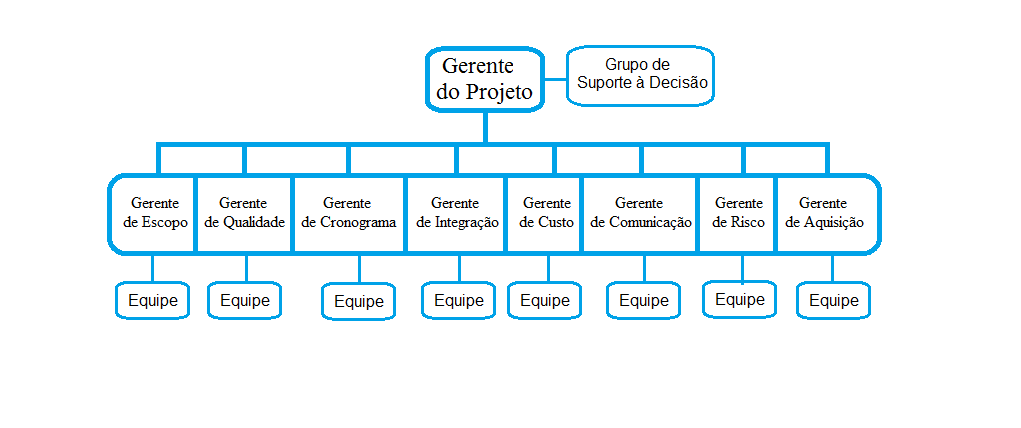
\includegraphics[scale=0.6]{Organograma}
\caption{Orgonograma do projeto}
\label{Rotulo}
\end{figure}
\FloatBarrier

 \section{Matriz de Responsabilidades}
 \FloatBarrier
 \begin{figure}[h]
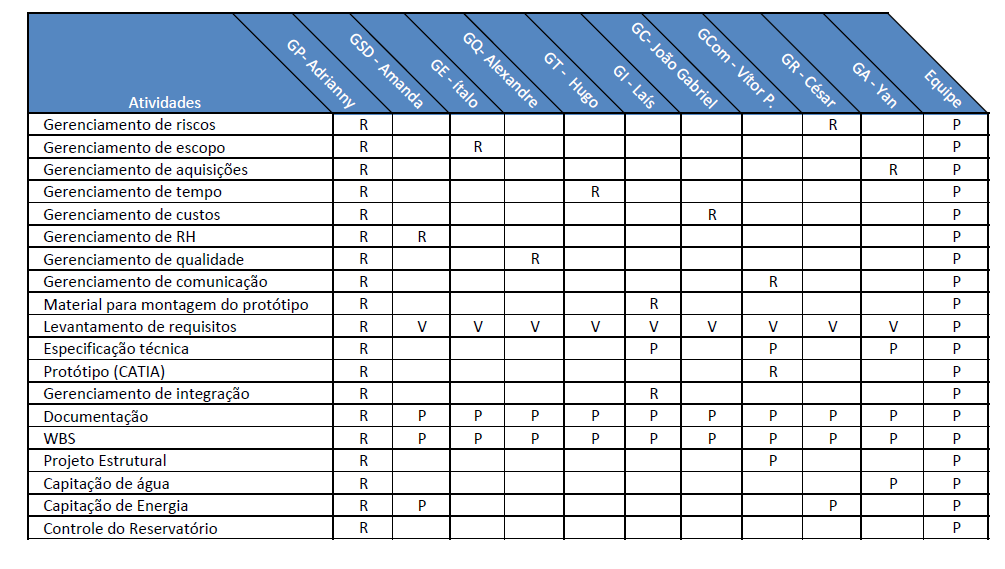
\includegraphics[scale=0.65]{matriz}
\label{matrizderesponsabilidades}
\caption{Matriz de Responsabilidades}
 \end{figure}

Legenda: R= Responsável; V= Valida; P= Participa.\\
  

\section{Novos recursos, realocação e substituição dos membros do time}
Em busca da realização dos objetivos do projeto, o gerente dos recursos humanos tem a responsabilidade e autoridade total para gerenciar e manejar todo o projeto, observando todo o ciclo de vida do mesmo, com o propósito de executar uma adequada alocação, realocação e substituição de recursos humanos, ou diversos, através do reconhecimento de competências, seleção, monitoração da alocação e avaliação dos recursos disponíveis ao projeto.

\section{Treinamento}
\begin{itemize}
 \item Capacitação da equipe do projeto: treinamento sobre Fundamentos de Gerenciamento de Projetos, onde deve ser abordada uma visão geral da metodologia, ferramenta, prática e cultura de gerenciamento de projetos.

 \item Desenvolvimento da tecnologia: treinamento interativo com o pessoal de produção, durante o qual se cria e desenvolve as instruções técnicas e de qualidade designadas. Consiste em apresentar um projeto de protótipo sobre a tecnologia utilizada no processo.

  \item Gestão da população de Acari: treinamento para capacitação de pessoal que interaja com a população e seus respectivos representantes políticos.
\end{itemize}

É de plena responsabilidade do Departamento de Recursos Humanos analisar as falhas de competência dos componentes do time verificados por meio das avaliações de desempenho para desenvolver treinamentos de qualificação e aperfeiçoamento.

\section{Avaliação de resultados do time do projeto}
Os sistemas de avaliação dos resultados do time do projeto são feitos a partir de reuniões semanais, nas quais são demonstradas e discutidas as evoluções até então, como também são definidos os próximos passos a serem dados, com base nas determinações já realizadas e nas orientações do que necessita ser feito.

\section{Bonificação}
Caso o projeto seja entregue em prazo estipulado e atendendo todos os requisitos de qualidade, a equipe do projeto receberá uma gratificação. O time terá uma confraternização social ao final do projeto.

\section{Freqüência da avaliação consolidada dos resultados do time}
Os resultados da frequência de avaliação serão apresentados em reuniões com o time, e divulgados nas plataformas de comunicação objetivando o esclarecimento de todos da equipe. Porém, haverão questões a serem discutidas individualmente com cada integrante do time.

\section{Alocação financeira para o gerenciamento de recursos humanos}
No gerenciamento de Recursos Humanos, os gastos adicionais relacionados ao setor devem ser alocados dentro das reservas gerenciais do projeto, sendo os responsáveis por administrar tais reservas os Gerentes de Projeto.

\section{Administração do plano de gerenciamento de recursos humanos}
\begin{enumerate}
 \item Responsável pelo plano:\\
 AMANDA LEITE DE CASTRO - GERENTE DE SUPORTE Á DECISÃO

ERIC VINÍCIUS LIMA BARBOSA - SUPLENTE DO RESPONSÁVEL DIRETO PELO PLANO DE GERENCIAMENTO DE SUPORTE À DECISÃO.
  \item Frequência de atualização do plano de gerenciamento de recursos humanos:\\
  O Plano de Gerenciamento de Recursos Humanos será revisto em reunião, datada para o dia 20/04/2015, e em suas reuniões subsequentes determinando e avaliando os resultados de cada membro do time.
\end{enumerate}

\section{Outros assuntos relacionados ao gerenciamento de recursos humanos do projeto não previstos nesse plano}
Todas as mudanças no quadro de gerenciamento dos Recursos Humanos devem ser apresentadas e discutidas em reunião sendo o Gerente de Recursos Humanos o responsável por tal avaliação. A responsabilidade de possíveis mudanças no quadro pessoal da equipe fica direcionada à comissão.

\section{Assinaturas}
\begin{center}
Data: \rule{0.5cm}{0.1mm}/\rule{0.5cm}{0.1mm}/\rule{1cm}{0.1mm}     \\
\rule{13cm}{0.1mm}\\
ADRIANNY VIANA DE ARAÚJO AMORIM – GERENTE DE PROJETO\\
\rule{13cm}{0.1mm}\\
AMANDA LEITE DE CASTRO - GERENTE DE RECURSOS HUMANOS

\end{center}
\end{document}
  
\chapter{Plano de Gerenciamento de Riscos}

  \documentclass[12pt,openright,oneside,a4paper,brazil]{abntex2}
\usepackage[utf8]{inputenc}
\counterwithout{section}{section}
\counterwithout{figure}{chapter}
\counterwithout{table}{chapter}
\setlength{\parindent}{1.3cm}
\usepackage{indentfirst}
\setlength{\parskip}{0.2cm}
\usepackage[bottom=2cm,top=3cm,left=3cm,right=2cm]{geometry}
\usepackage{graphicx}
\graphicspath{{figuras/}}
\usepackage{placeins}

%opening
\title{}
\author{}

\begin{document}


\textual
\begin{center}
 {\large Plano de gerenciamento de riscos}\\[0.2cm]
 {Planta de abastecimento de água potável a partir da umidade do ar}\\
 \end{center}
 
 \section{Histórico de Alterações}
\begin{table}[h]
\centering
\begin{tabular}{|c|c|p{6cm}|p{5cm}|}

Data & Versão & Descrição & Responsável\\
\hline                               
17/04/2015 & 0.0 & Criação do Plano de Gerenciamento das comunicações & Cesar Antonio Marques Junior, Jonnatas Lennon Lima Costa, Victor Borges.
\\
\hline
24/04/2015 & 1.0 & Alteração nos itens VII, VII e X & Cesar Antonio M. Júnior.\\
\hline
\end{tabular}
\end{table}

\section{Objetivo}
O objetivo desse plano é estabelecer um processo de gerenciamento de riscos do projeto.

\section{Descrição dos processos de gerenciamento de riscos}
Dentre os processos de gerenciamento de riscos deve-se frisar pela identificação e  analise qualitativa dos riscos, para assim obter ferramentas de respostas eficazes aos ricos evidentes, assim sendo os artefatos gerados neste projeto serão.
\begin{itemize}
\item Plano de gerenciamento de risco.
\item Identificação de risco.
\item Analise quantitativa de risco.
\item Analise qualitativa de tisco.
\item Planejamento de resposta aos riscos.
\end{itemize}

\section{EAR – Estrutura Analítica de Riscos para identificação dos riscos}
\begin{figure}[h]
\begin{center}

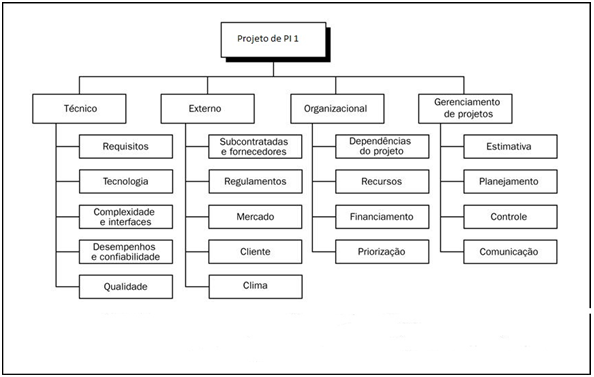
\includegraphics[scale=0.65]{ear}
\label{ERR}

\end{center}
\end{figure}
\FloatBarrier

\section{Qualificação dos riscos}
Os riscos identificados serão qualificados na sua probabilidade de ocorrência e impacto nos resultados, conforme tabela a seguir:

Probabilidade:
\begin{table}[h]
\centering
\begin{tabular}{|c|c|c|}

  & Nível & Descrição\\
\hline                               
1 & baixa & Impedimento devido a licenças ambientais. \\
\hline
2 & alta & Alto custo dos componentes integrantes no aparelho.\\
\hline
3 & alta & Pouco tempo para o desenvolvimento de um projeto altamente complexo.\\
\hline
4 & media & Pouca vasão de agua gerada, pelo aparelho. \\
\hline
\end{tabular}
\end{table}

Impacto:
\begin{table}[h]
\centering
\begin{tabular}{|c|c|p{13.3cm}|}

  & Nível & Descrição\\
\hline                               
1 & alta & Caso ocorra havera a paralização da execução do projeto. \\
\hline
2 & alta & Caso ocorra podera inviabilizar o projeto devido o alto custo do aparelho a ser desenvolvido.\\
\hline
3 & alta & Não ocorrerar grande impactos no projeto.\\
\hline
4 & media & Ocorrerar inviabilidade finaceira sobre a implementação. \\
\hline
\end{tabular}
\end{table}

Prioridade: Probabilidade X Impacto
\begin{figure}[h]
\begin{center}

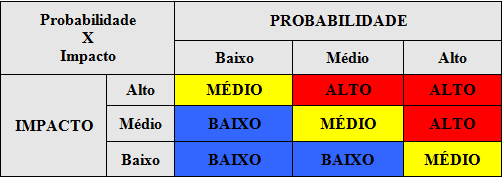
\includegraphics[scale=0.65]{prioridade}
\label{Prioridade}
\end{center}
\end{figure}
\FloatBarrier

\section{Quantificação dos riscos}
Análise quantitativa dos riscos tem como objetivo mensurar a probabilidade de ocorrência dos riscos, suas conseqüências e estimar as implicações no projeto.

A análise quantitativa de riscos deve ser repetida após o planejamento de respostas a riscos, e também como parte do monitoramento e controle de riscos, para determinar se o risco total do projeto diminuiu de forma satisfatória. As tendências podem indicar uma necessidade de aumento ou diminuição das ações de gerenciamento de riscos.

Serão usadas técnicas como a análise de árvore de decisão e a simulação de Monte Carlo para:
\begin{itemize}
\item Quantificar os possíveis resultados do projeto e suas probabilidades.
\item Avaliar a probabilidade de atingir objetivos específicos do projeto.
\item Identificar os riscos que exigem mais atenção quantificando sua contribuição relativa para o risco total do projeto.

\end{itemize}

\section{Sistema de Controle de mudanças de riscos}
As mudanças surgirão basicamente da comparação dos resultados obtidos com os resultados esperados. Durante as reuniões os pontos analisados são levantados para discussão entre os integrantes do grupo, dessa forma o resposável por tal atividade e os envolvidos poderão buscar a melhor alternativa de contenção para os riscos avaliados. 

\section{Reserva de contingência}
\begin{table}[h]
\centering
\begin{tabular}{|c|c|}
Cargo & Reservas de contingência\\
\hline
Gerente de projeto & Até R\$ 2.000\\
\hline
Compras com equipamentos & Até R\$ 3.000\\
\hline
Pesquisa e desenvolvimento & Até R\$ 500\\
\hline
\end{tabular}
\end{table}

Esta autonomia baseia-se na nas diretrizes do plano de gerenciamento dos riscos, de modo à oferecer uma resposta rápida, as ações que ocasionariam algum risco, com base em ocorrência das ações. 
\section{Frequência de avaliação dos riscos do projeto}
Seguindo o cronograma de atividades do projeto, a avaliação dos riscos será feita conforme a entrega das atividades de cada área do projeto, estando sujeita à aprovação dos envolviodos e do responsável por tal atividade.

\section{Alocação financeira para o gerenciamento de riscos}
Deve-se ter um capital em reserva, a fim de garantir um bom planejamento na gestão de mudanças de caráter corretivo ou preventivo, assim sendo deve-se manter um sistema de gerenciamento dos os recursos gerais do projeto, mantendo uma parcela para sanar esta necessidade, mantendo a autonomia nas demais áreas do projeto.
Caso esta reserva atinja o limite ou esgote deve ser revisto todas as demais alocações, com o intuito balancear o orçamento do projeto.

\section{Administração do plano de gerenciamento de riscos}
\begin{enumerate}
\item Responsável pelo plano:
\begin{itemize}
\item CESAR ANTONIO MARQUES JÚNIOR.
\item JONNATAS LENNON LIMA COSTA.
\end{itemize}
\item Frequência de atualização do plano de gerenciamento de riscos

O plano de gerenciamento de riscos será atualizado durante as reuniões que se seguem após a entrega das atividades programadas
\end{enumerate}

\section{Outros assuntos relacionados ao gerenciamento de riscos do projeto não previstos nesse plano}
Qualquer desvio no ambiente como mudanças climáticas que poderia deixar de favorecer o aproveitamento da umidade do ar para extração da água é um fator de insucesso para o projeto. Esses fatores serão contornados mudando de tecnologia e/ou aproveitando os picos de melhor umidade do ar para retirar a água.

\section{Assinaturas}
\begin{center}
Data: \rule{0.5cm}{0.1mm}/\rule{0.5cm}{0.1mm}/\rule{1cm}{0.1mm}     \\
\rule{13cm}{0.1mm}\\
ADRIANNY VIANA DE ARAÚJO AMORIM – GERENTE DE PROJETO\\
\rule{13cm}{0.1mm}\\
CESAR ANTONIO MARQUES JÚNIOR - GERENTE DE RISCOS


\end{center}
\end{document}
  
\chapter{Documento de visão: Sistema de monitoramento do processo de captação e distribuição da água.}

   \section*{\centerline{Planta de abastecimento da água através da umidade do ar.}}
 \centerline{ \textbf{Sistema de monitoramento do processo de captação e distribuição da água.}}
 \centerline{\textbf{Documento de visão técnica.}}

 
 \textbf{HISTÓRICO}
 \begin{longtable}{|m{2.8cm}|m{1.5cm}|m{4.2cm}|m{3.5cm}|}
  \hline
\textbf{Data} & \textbf{Versão} & \textbf{Descrição} & \textbf{Autor}\\
  
  \hline
  18/05/2015 & 0.1 & Criação do documento & Hugo Martins\\
  \hline
  18/05/2015 & 0.2 & Definição da descrição do problema e de alguns requisitos do sistema & Alexandre Torres,  Hugo Martins, Italo Paiva, Jonnatas Lennon e Karine Valença\\
  \hline
  18/05/2015 & 0.3 & Edição no documento geral & Hugo Martins e Italo Paiva\\
  \hline
  21/05/2015 & 0.4 & Criação dos requisitos do sistema & Alexandre Torres, Hugo Martins, Italo Paiva, Jonnatas Lennon e Karine Valença\\
  \hline
  21/05/2015 & 0.5 & Edição no documento geral & Alexandre Torres\\
  \hline
  23/05/2015 & 0.6 & Edição no documento geral & Hugo Martins\\
  \hline
  25/05/2015 & 0.7 & Criação dos requisitos não funcionais & Alexandre Torres,  Jonnatas Lennon, Karine Valença\\
  \hline
  26/05/2015 & 0.8 & Modificação dos requisitos funcionais & Alexandre Torres\\
  \hline
  27/05/2015 & 0.9 & Alterações gerais  e finalização do documento & Alexandre Torres\\
  \hline
  16/06/2015 & 1.0 & Reestruturação do documento & Hugo Martins\\
    \hline
  20/06/2015 & 1.0 & Incrementando novos requisitos funcionais derivados dos três subsistemas definidos & Hugo Martins, Alexandre Torres e Jonnatas Lennon\\
  \hline
 \end{longtable}
 
  \section{INTRODUÇÃO}
  Como tentativa de amenizar os problemas gerados pela falta de água potável na cidade de Acarí - RN, foi proposto um sistema 
  capaz de gerar água de boa qualidade a partir da umidade do ar. Para o correto funcionamento desse sistema é necessário um 
  software capaz de permitir o monitoramento da água.
  
  O objetivo primário do software proposto será o monitoramento da qualidade e disponibilidade da água. Além disso, ele 
  disponibilizará outras informações relacionadas a tecnologia proposta referentes, por exemplo, à turbina, à casa de 
  controle, ao monitoramento da adição de sais.
  
  \section{DESCRIÇÃO DO PROBLEMA}
  Encontra-se abaixo a tabela com a descrição do problema identificado:
  
   \begin{longtable}{|m{5.0cm}|m{11.2cm}|}
  \hline
\textbf{O problema da:} & Falta de monitoramento do processo de captação e distribuição da água.\\
  \hline
\textbf{Que afeta:} & Além dos cidadãos da cidade de Acarí - RN, também afeta os envolvidos no desenvolvimento do projeto da planta de abastecimento da água através da umidade do ar.\\
  \hline
\textbf{Cujo o Impacto é:} & A não garantia do correto funcionamento do sistema, podendo causar problemas à saúde humana e a inviabilidade do projeto.\\
  \hline
\textbf{Uma solução seria:} & A implementação de um software para o monitoramento do processo de captação e distribuição da água.\\
  \hline
 \end{longtable}
   
  \section{DESCRIÇÕES DOS ENVOLVIDOS E USUÁRIOS}
  Os stakeholders envolvidos no projeto de software são a equipe de desenvolvimento do projeto, mais diretamente a equipe 
  formada pelos integrantes da engenharia de software, os professores orientadores do projeto, os técnicos que serão usuários 
  do sistema e a população que vai se beneficiar do mesmo.
  
  \subsection{Resumo dos Envolvidos}
  A equipe composta por 27 alunos do grupo 1 da disciplina Projeto Integrador I da Universidade de Brasília, Campus Gama 
  no 1º semestre de 2015, técnicos que ficarão responsáveis pelo acompanhamento do sistema, os professores orientadores e 
  da população da cidade de Acarí – RN, mais especificamente no bairro Vereador Tarcísio Bezerra Galvão.
  
  \subsection{Resumo dos Usuários}
  Os técnicos responsáveis pelo acompanhamento do sistema, irão monitorar os dados referentes ao  processo de captação e 
  distribuição da água gerados pelo sistema.
  
  \subsection{Ambiente dos Usuários}
  O sistema será implantado na casa  de Controle da planta de abastecimento da água. Esta casa de controle objetiva manter que 
  todo o sistema esteja funcionando da maneira esperada.
  
  \subsection{Ambiente das Principais Necessidades dos Envolvidos ou Usuários}
  A equipe deve assegurar que a água extraída pela planta esteja em um nível considerável para consumo. Caso não esteja, o 
  problema causador deve ser mitigado evitando que ocorra novamente. O técnico também abastecerá o reservatório de sais 
  utilizados na mistura com a água caso esteja com uma pequena quantidade.
  
  \section{VISÃO GERAL DO PRODUTO}
  
  \subsection{Perspectiva do Produto}
  Esse software é um componente do sistema proposto de geração de água potável a partir da umidade do ar. A sua finalidade 
  principal é o monitoramento do sistema como um todo. Esse sistema está dividido em três subsistemas: 
  
  1. Subsistema de monitoramento mecânico e lógico das turbinas eólicas.
  2. Subsistema de monitoramento da qualidade da água.
  3. Subsistema de monitoramento do reservatório de distribuição.
  
  Alguns dos dados referentes ao monitoramento mecânico e lógico das turbinas que serão monitorados pelo software são: as temperaturas 
  internas, a quantidade de energia gerada por cada turbina e a velocidade de rotação das pás. 
  
  O subsistema de monitoramento da qualidade da água analisará, por exemplo, a quantidade de sais na água, o pH, a condutividade e a 
  turbidez, além de informar dados referentes ao volume de água disponível no reservatório.
  
  O subsistema de monitoramento do reservatório de distribuição deve monitorar o volume da água gerada pelas turbinas, armazenadas
  no reservatório e distribuídas para a população.
  
  Percebe-se, portanto, que o software proposto visa, basicamente, possibilitar o monitoramento de uma série de aspectos relacionados a 
  tecnologia de captação de água a partir da umidade do ar.
  
  
  \subsection{Suposições e Dependências}
  É possível que haja alterações futuras no software proposto, principalmente, relacionadas a integração com eletrônica. Alterações 
  nos componentes eletrônicos afetam diretamente o software proposto.
  
  
  \section{RECURSOS DO PRODUTO}
  Este item traz todos os recursos referentes ao produto: Os requisitos funcionais, os não funcionais e as restrições referentes 
  ao sistema. Cada um desses requisitos possui um código de identificação para facilitar a rastreabilidade, a sua descrição e 
  o seu nível de prioridade que são prioridade alta, média ou baixa e abaixo está estabelecido o significado de cada uma 
  destas prioridades.
  
  \textbf{Alta:}  O sistema só funcionará de maneira eficaz caso este requisito esteja sendo atendido.
  \textbf{Média:} O sistema pode funcionar caso este requisito não seja atendido.
  \textbf{Baixa:} O sistema funcionará 	normalmente caso este requisito não seja atendido.
  
  
  \subsection{Requisitos Funcionais}
  
  Os requisitos do sistema de monitoramento do processo de captação e distribuição da água foi dividido em 
  três subsistemas que estão listados abaixo junto a cada um de seus requisitos:
  \pagebreak
  
  \textbf{1. Monitoramento mecânico e lógico das turbinas eólicas}
  
  \begin{longtable}{|m{3.0cm}|m{7.5cm}|m{3.5cm}|}
   \hline
\textbf{Código} & \textbf{Descrição} & \textbf{Prioridade}\\
\hline
RF01 & O sistema deve permitir o monitoramento dos dados recebidos pelo acelerômetro (dados referentes à vibração da turbina). & Alta\\
\hline
RF02 & O sistema deve permitir o monitoramento dos dados recebidos pelo sensor Hall (dados referentes a velocidade de rotação das pás da turbina). & Alta\\
\hline
RF03 & O sistema deve monitorar os dados recebidos pelo sensor de temperatura presente no compartimento do condensador. & Alta\\
\hline
RF04 & O sistema deve permitir o monitoramento dos dados recebidos pelo sensor de temperatura presente no compartimento do condensador. & Alta\\
\hline
RF05 & O sistema deve permitir o monitoramento dos dados recebidos pelo sensor de temperatura presente no compartimento próximo ao rotor. & Alta\\
\hline
RF06 & O sistema deve permitir o monitoramento dos dados recebidos pelo anemômetro (dados referentes a velocidade e direção do vento). & Alta\\
\hline
RF07 & O sistema permitir o monitoramento da carga das baterias presentes na turbina. & Alta\\
\hline
RF08 & O sistema deve permitir a visualização de todos os dados recebidos acerca do funcionamento da turbina. & Alta\\
\hline
RF09 & O sistema deve gerar mensagens de alerta para níveis extremos de algum dado recebido. & Alta\\
\hline
RF10 & O sistema deve permitir o monitoramento da distribuição da água das turbinas para o reservatório de tratamento. & Alta\\
\hline
RF11 & O sistema deve permitir o controle da válvula do reservatório de água presente em cada turbina. & Alta\\
\hline
RF12 & O sistema deve permitir o monitoramento do nível de água do reservatório da turbina. & Alta\\
\hline
   
  \end{longtable}

  \textbf{2. Monitoramento da qualidade da água}
  
    \begin{longtable}{|m{3.0cm}|m{7.5cm}|m{3.5cm}|}
      \hline
\textbf{Código} & \textbf{Descrição} & \textbf{Prioridade}\\
\hline
RF13 & O sistema deve permitir o monitoramento dos dados referente ao pH da água. & Alta\\
\hline
RF14 & O sistema deve permitir o monitoramento dos dados referente a condutividade elétrica da água. & Alta\\
\hline
RF15 & O sistema deve permitir o monitoramento dos dados referente a turbidez da água. & Alta\\
\hline
RF16 & O sistema deve gerar mensagens de alerta para níveis de sais fora dos parâmetros. & Alta\\
\hline
RF17 & O sistema deve permitir a visualização de todos os dados recebidos acerca dos dados referentes aos sais. & Alta\\ 
\hline
RF18 & O sistema deve permitir o anexo dos relatórios referentes a análise química da água (obtidos pela empresa terceirizada). & Alta\\
\hline
RF19 & O sistema deve permitir a consulta dos relatórios referentes a análise química da água (obtidos pela empresa terceirizada). & Alta\\
\hline
RF20 & O sistema deve permitir o monitoramento do nível de água do reservatório de tratamento. & Alta\\
\hline
RF21 & O sistema deve permitir o controle da válvula que liga o reservatório de tratamento ao reservatório de distribuição. & Alta\\
\hline
RF22 & O sistema deve permitir o controle da válvula que liga o reservatório à rede. & Alta\\
\hline
  \end{longtable}
  \pagebreak
  \textbf{3. Monitoramento do reservatório de distribuição}
  
    \begin{longtable}{|m{3.0cm}|m{7.5cm}|m{3.5cm}|}
      \hline
\textbf{Código} & \textbf{Descrição} & \textbf{Prioridade}\\
\hline
RF23 & O sistema deve permitir o monitoramento do nível da água no reservatório. & Alta\\
\hline
RF24 & O sistema deve permitir o monitoramento da quantidade de água distribuída para a população. & Alta\\
\hline
RF25 & O sistema deve permitir o controle da válvula de distribuição da água para a rede da cidade. & Alta\\
\hline
RF26 & O sistema deve permitir o controle da válvula que encaminha a água para engarrafamento. & Alta\\
\hline
RF27 & O sistema deve permitir o cadastro de cidadãos beneficiados pela água gerada. & Alta\\
\hline
RF28 & O sistema deve permitir a consulta de cidadãos beneficiados pela água gerada. & Alta\\
\hline
RF29 & O sistema deve gerar relatórios referente ao número de cidadãos beneficiados pela água gerada. & Alta\\
\hline
  \end{longtable}
  
  Além disso, o sistema possui alguns requisitos gerais:
  
    \begin{longtable}{|m{3.0cm}|m{7.5cm}|m{3.5cm}|}
      \hline
\textbf{Código} & \textbf{Descrição} & \textbf{Prioridade}\\
\hline
RF30 & O sistema deve possuir um controle de acesso aos dados. & Média\\
\hline
RF31 & O sistema deve permitir gerar relatórios com dados referentes ao monitoramento da qualidade da água. & Média\\
\hline
RF32 & O sistema deve permitir gerar relatórios com dados referentes ao Monitoramento mecânico e lógico das turbinas eólicas. & Média\\
\hline
RF33 & O sistema deve permitir gerar relatórios com dados referentes ao Monitoramento do reservatório de distribuição. & Média\\
\hline
RF34 & O sistema deve permitir a impressão de relatórios com dados referentes ao monitoramento da qualidade da água. & Média\\
\hline
RF35 & O sistema deve permitir a impressão de relatórios com dados referentes ao Monitoramento mecânico e lógico das turbinas eólicas. & Média\\
\hline
RF36 & O  sistema deve permitir a impressão de relatórios com dados referentes ao Monitoramento do reservatório de distribuição. & Média\\
\hline

  \end{longtable}
  
  \subsection{Requisitos Não Funcionais}
  Este item traz a especificação dos requisitos que dão suporte para a correta execução dos requisitos funcionais e indicam quais são as limitações 
  do sistema e do seu desenvolvimento.
  
  \subsection{Usabilidade:}
  O sistema deve obedecer às metas de usabilidade. Além disso, ele deve possuir um sistema de ajuda para responder eventuais duvidas do usuário.
  
  \subsection{Confiabilidade:}
  O sistema deverá estar disponível 24h por dia. Além disso, o sistema não deve ser tolerante em falhas relacionados aos critérios de qualidade da água.

  \subsection{Portabilidade:}
  O sistema deve manter o seu correto funcionamento nos sistemas operacionais Windows XP SP3 ou superior, nos sistemas operacionais Linux e Mac OS.
	
  \subsection{Linguagem:}
   sistema será desenvolvido em C\#/C++.

  \subsection{Restrições do Sistema}
  
     \begin{longtable}{|m{4.0cm}|m{12.2cm}|}
  \hline
\textbf{Código} & \textbf{Descrição}\\
  \hline
RS1 & O sistema deverá estar associado a um banco de dados local, onde ficarão armazenados os dados obtidos.\\
  \hline
RS2 & O software deverá funcionar continuamente, sem interrupções.\\
  \hline
RS3 & O software deve ser desenvolvido deverá ser desenvolvido na linguagem C\# ou C++.\\
  \hline
RS4 & O sistema deve ser capaz de interagir com os microprocessadores definidos.\\
  \hline
 \end{longtable}
  
  \section{RÓTULO E EMBALAGEM}
  
  O sistema deve possuir a logo do projeto representado na figura abaixo.
  
    \begin{figure}[!h]
    \centering
    
\includegraphics[scale = 0.2]{editaveis/figuras/logo}
    \label{logo}
    \caption{Logomarca do projeto}
   \end{figure}
   \FloatBarrier
 


\chapter{Diagrama Fishbone}
  
  \begin{figure}[!h]
    \centering
    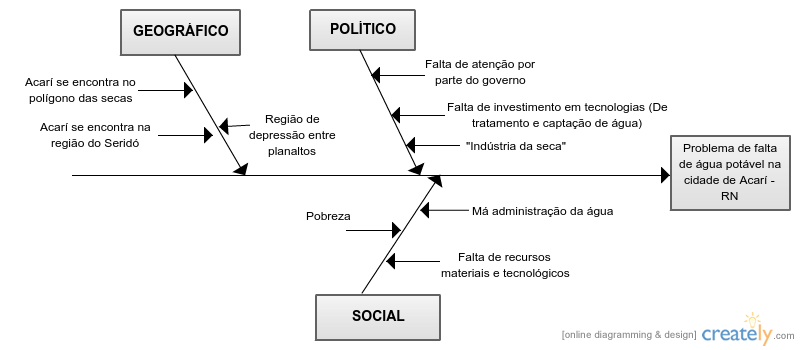
\includegraphics[scale = 0.7, angle = 90]{editaveis/figuras/fishbone}
    \label{fishbone}
    \caption{Diagrama de Fishbone}
   \end{figure}
   \FloatBarrier

\end{anexosenv}

